\chapter{The Quest for a Quantum Computer}
\label{sec:quest}
Before delving into the question of how we might build a quantum computer, it is worth taking a step
back and exploring the question of what brought us as a scientific community to the point where
it is seen as a priority to build one. The answer to that requires us to delve briefly into
the world of computational complexity theory, and to examine what it means to solve problems "efficiently".
Although the genesis of computation can be traced back to pioneering works by people such as Charles Babbage
and Ada Lovelace in the early 1800's \cite{Bowden:1953:FTS:1102044}, it was not until the early 1900's that
machines we might recognize as computers were constructed. Based on delicate vacuum tubes and mechanical relays,
and often taking up full rooms, their inherent fragility and bugginess posed formidable obstacles to scaling.
It was not until the mid-1900's that the field took off with two pivotal discoveries. The first
was the construction of the first transistor in 1947, credited to Bardeen, Brittain and Schockley and for which
they were awarded the Nobel Prize in 1956 \cite{nobel1956}. This was followed by the creation of integrated circuits by Jack Kilby
in 1959, for which he was awarded the Nobel Prize in the year 2000 \cite{nobel2000}. With these two inventions, a remarkable
surge in computational power occurred. This surge is embodied in Moore's law, which described an annual
doubling in the number of transistors that it would be possible to fit on a single integrated circuit \cite{4785860}.
And with this doubling came an exponential growth in the computation power that we had available to us.

Along with this growth came an obvious question. What exactly can these computers do? What sorts of
problems will we be able to solve with our ever-growing bundle of transistors? To answer this question, we need to
think about how many steps it takes to run various algorithms. Take for example the question of looking
for a single item $x_T$, in a list $L = \{x_0, x_1, ..., x_n\}$ with $n$ items in it. Assuming the list
is in an unknown order, to find the location of the item $x_T$, we need to look at each item in the list
in turn. If the length of the list were doubled to $2n$ items, it would take twice as many comparisons to
look through the list. Tripled would be three times. The amount of time it takes to find an item in the
list is \emph{linear} in the length of the list. We can write this scaling mathematically using big-$\mathcal{O}$
notation: searching for an item in a list is $\mathcal{O}(n)$.

What about a slightly more complicated problem. What if we want to check whether any item $x_i$ appears
in the list twice? To run this algorithm, we can run the above algorithm for each item in the list, setting the
target to $x_T = x_0$, then $x_T = x_1$ and so forth, and checking whether we find each item two or more
times. So for $n$ items in the list, we run through the list $n$ times, so the number of steps to run
the algorithm scales as $\mathcal{O}(n^2)$. That is, if the length of the list is doubled, it takes
four times as long, so the scaling is \emph{quadratic}.
In this way, we can classify algorithms into various complexity classes. For example, sorting a list
of $n$ items is, in the best case, $\mathcal{O}(n \log(n))$. Solving the travelling salesman problem (TSP) is
$\mathcal{O}(n^2 2^n)$. Ideally we would like to group problems into various complexity classes. For example,
we can group problems that have at worst a polynomial complexity, i.e. $\mathcal{O}\left(f(n)\right)$ where $f(n)$
is a polynomial into the complexity class \cc{P} (for polynomial). We will call these problems \textbf{efficiently
computable}. Other problems may grow at worst exponentially in the size of the problem. We can group all
of those problems into the complexity class \cc{EXP}. These problems, and indeed any problem that has a difficulty
that grows faster than a polynomial in the size of the problem are said to be inefficient to compute.

Of course, you might say, well what sort of operations do we allow our computers to do in a single step?
If I say that my computer can solve the TSP in a single step, then the complexity of that problem reduces trivially to
$\mathcal{O}(1)$. The answer is not so trivial --- it is limited by the laws of physics. What sorts
of computation do they allow? To answer this question, Alan Turing and Alonzo Church came up with the notion of
the Turing Machine, a universal model for a physical computational device, and with it stated the Church-Turing
hypothesis:

\begin{displayquote}[\cite{turingthesis}]
  "a function is effectively calculable if its values can be found by some purely mechanical process".
  We may take this literally, understanding that by a purely mechanical process one which could be carried out by a machine.
\end{displayquote}

To paraphrase, this stated that anything a Turing machine could do, a computer could do too, and anything
it \emph{can't} do, no computer can. It wasn't long before this was extended to the strong Church-Turing
hypothesis, which states \textquote[\cite{kaye2007an}]{A probabilistic Turing machine can efficiently simulate any
realistic model of computation}\footnote{Note we had to add the word "probabilistic" to the statement of the strong
 Church-Turing hypothesis. This was due to the discovery of a new complexity class, bounded-error probabilistic polynomial (\cc{BPP}),
 which includes problems  we can solve with $> 2/3$ chance in polynomial time. By running these algorithms repeatedly, we can solve
 problems to within a small error $\epsilon$ in polynomial time.}.
Note the addition of the term \emph{efficiently}. This prescribes that for any
operation we could add to any physical computer, we can get at most a polynomial speedup. Since
a polynomial $P(n)$ divided by another polynomial $Q(n)$ is still a polynomial, and anything that grows faster
than a polynomial $E(n)$ divided by a polynomial $Q(n)$ still grows faster than a polynomial, we have
a universal definition for problems that are efficient to solve and those that aren't.
\footnote{Of course, since we're continually coming up with better algorithms to solve hard problems,
the set of algorithms that are efficient to solve seems to keep growing!}


\begin{figure}
  \includegraphics[width=0.7\linewidth]{MooresLaw}
  \caption[Moore's Law and the end of exponential scaling]
  {Graph of the number of transistors per chip, their clock speed, and their
  thermal design power plotted on a log scale against time. Although the number of transistors per chip
  continues to grow exponentially, the clock speed and power per chip have plateaued in the early 2000s.
  Reproduced with permission from \cite{cross_2016}.}
  \label{fig:mooreslaw}
\end{figure}

So we've established what sorts of problems a computer can solve efficiently, and we've also noted the
exponential growth in the number of transistors on a chip. As long as both of these facts remain true, we
should only have to wait a few years before our computers become twice as powerful and problems that were
previously intractable fall within our grasp. Unfortunately, any exponential scaling must eventually fail,
and so it was for ICs for two key reasons: power and transistor size. As we made our transistors smaller,
we stopped seeing a concomitant efficiency increase, and all of a sudden, the power density of our ICs
became a limiting factor. To halt this increase, we had to reduce power dissipation, and the
only way we saw how was by capping the clock speed of our computers, which we can see in Fig.~\ref{fig:mooreslaw}
has plateaued since the early 2000s. Moreover, the smaller our transistors became, the more costly they became
to make. Even Moore's law, which has stubbornly held past the expectations of most scientists, must eventually
end as we bump up against the sizes of atoms. It seems unlikely that there is much room below Samsung's
recently announced \SI{3}{\nano\meter} node, so if we want to bring more problems into the fold of the
possible, it seems like the strong Church-Turing hypothesis must give.

It was in this context that Feynmann gave his seminal address, noting that as far as we can tell, simulating
quantum systems falls outside of the set of problems that are efficiently solveable on classical computers \cite{Feynman1982}.
However, as long as we can manipulate quantum systems, we should also be able to set up a "quantum
simulator" to see how a quantum system behaves. If this turned out to be the case, then the strong
Church-Turing hypothesis would be violated\footnote{Despite this violation, as far as we know the original
Church-Turing hypothesis still holds. No previously uncomputable function became computable with the addition
of quantum physics.}! Here was nature efficiently simulating a system that as far as we know, a Turing machine
can't. It was David Deutsch who in 1985 formalized the idea of a quantum Turing machine \cite{doi:10.1098/rspa.1985.0070},
and laid out the Deutsch-Church-Turing hypothesis, which as far as we know holds to this day:

\begin{displayquote}
  A quantum Turing machine can efficiently simulate any realistic model of computation.
\end{displayquote}

\begin{figure}
  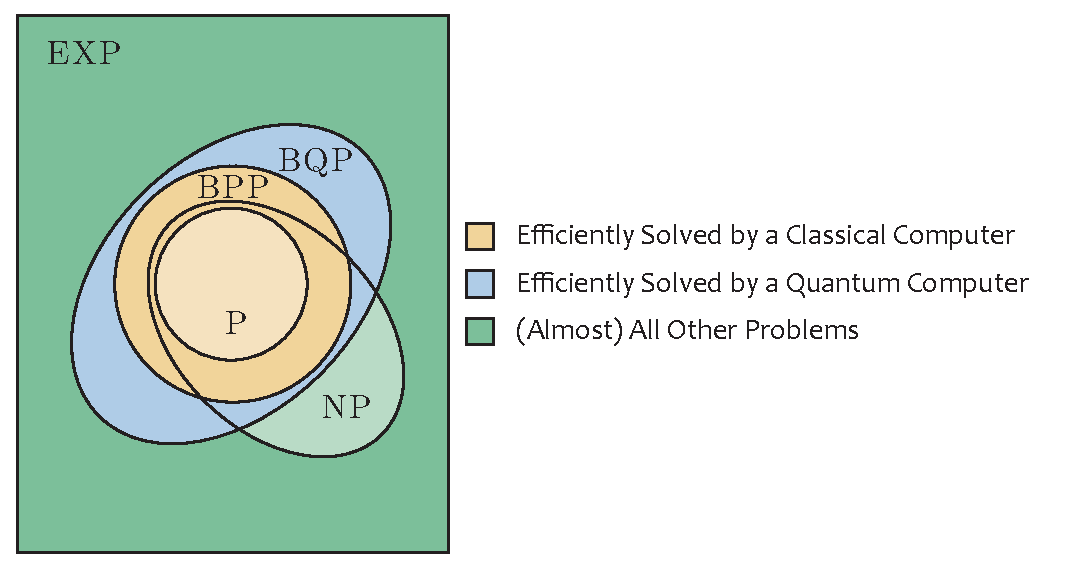
\includegraphics[width=0.85\linewidth]{ComplexityClasses}
  \caption[Relationship between various complexity classes]
  {Relationship between the various complexity classes that we've discussed. The class
  \cc{BPP} includes all problems that a classical computer can solve efficiently (including
  everything that can be calculated in polynomial time). \cc{BQP} are all problems a quantum computer can
  solve efficiently (which includes everything a classical computer can do). Finally, problems that scale exponentially
  with input size, labelled \cc{EXP}, are (almost) all other problems that are computable. The class
  \cc{NP} is also included on this figure as it is one that often comes up in the context of complexity,
  if for no other reason than to emphasize that a quantum computer \emph{cannot} solve all problems in
  this class.}
  \label{fig:complexity}
\end{figure}

With that, we finally define the class of problems that we might be able to solve efficiently if we
can build a quantum computer --- Bounded-Error Quantum Polynomial-Time or \cc{BQP}. As far as we know,
this class includes interesting problems that a classical computer could not efficiently solve. Problems
such as Shor's algorithm for prime factorization \cite{Shor} or estimating the ground state of molecules with
the Variational Quantum Eigensolver algorithm \cite{ncomms5213} have no known efficient classical algorithm
but could profoundly impact society if they are solvable. It is the promise of solutions to these problems
that drive the search for a quantum computer; however, the challenges of realizing one remain formidable. To close
out our discussion of complexity classes, I've summarized the relationship between complexity classes in
Fig.~\ref{fig:complexity}. A point I'd like to emphasize is that although \cc{BQP} is larger than \cc{P}
or \cc{BPP}, it certainly does not enclose all problems, especially those in \cc{EXP}. Although a
quantum computer may offer an exponential speedup on a subset of algorithms, it will not give us an exponential
speedup in the general case.

The remainder of this chapter aims to lay out the fundamentals of quantum computing and how we might realize
them in a semiconductor system. In Section~\ref{sec:qc}, I go through a quick introduction to the concepts
underlying quantum computation. In Section~\ref{sec:qcinsm}, I will detail several methods by which we might
realize a qubit in a semiconductor. Finally, in Section~\ref{sec:char}, I will outline the characterization of a 2DEG,
the system in which we make qubits.

\section{A Quick Introduction to Quantum Computing}
\label{sec:qc}
To build a quantum computer, we start by defining the notion of a quantum bit (qubit), which
serves as the quantum analog to the classical bit. To review, a classical \textbf{bit} is a "piece" of information
that can either take the value 0 or 1. It represents the fundamental unit of computation in digital computers.
We can take individual bits, and combine them to form a \textbf{register}, whose state is defined as
the state of each bit in the register. For example, two bits can take up to 4 different
values: 00, 01, 10, 11. Three bits can take up to 8 values, and $N$ bits can take up to $2^N$ values, however
to give the state of a register all we have to do is list the state of each bit in that register, a total of $N$ states.
By choosing various encodings of values, we can map numbers, letters, and other symbols onto these registers
and perform computations on them. For example, we can map positive integers onto registers using a base-2 number
system, as in Fig.~\ref{fig:binary}, or letters using a mapping such as ASCII, which assigns letters to 8-bit registers.
Other mappings exist for negative numbers (such as a mapping called two's complement), numbers with
decimal points (such as IEEE floating point), complex numbers and so forth.

\begin{figure}
  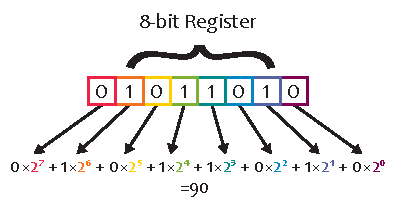
\includegraphics[width=0.75\linewidth]{Binary}
  \caption[Binary coding]
  {We can encode information in a register in many ways. One encoding for positive numbers is to use a base-2
  positional system, like above, where the binary register \texttt{01011010} is mapped to the number 90.}
  \label{fig:binary}
\end{figure}

\subsection{The Qubit}
A \textbf{qubit} is similar to a bit in that it has two states, $\ket{0}$ and $\ket{1}$, except unlike a bit, it is specified
by a 2-dimensional vector, and evolves according to the rules of quantum mechanics. Due to the uniquely quantum
mechanical property of \textbf{superposition}, we can no longer write the state of a single qubit (which we will
denote $\psi$) as either $\ket{0}$ or $\ket{1}$. Instead, we must write down the vector sum of the two states,
which we define as follows:
\begin{align}
  \label{eqn:basisstates}
  \ket{0} = \svec{1\\0} && \ket{1} = \svec{0\\1}
\end{align}
\begin{equation}
  \ket{\psi} = \alpha \ket{0} + \beta \ket{1} = \svec{\alpha\\\beta}
\end{equation}
where $\alpha$ and $\beta$ are complex numbers. If we were to take a measurement of this quantum state,
rather than getting back the value of this vector sum, we would measure the $\ket{0}$ state with probability
$|\alpha|^2$ and the $\ket{1}$ state with probability $|\beta|^2$. Since probabilities must sum to one, we also
get a normalization condition: $|\alpha|^2 + |\beta|^2 = 1$. The quantities $\alpha$ and $\beta$ are called
probability amplitudes, and they can take both positive and negative complex values\footnote{Interestingly, the "complex"
  part of that state is unnessecary to get the extra computing power
  of a quantum computer \cite{doi:10.1142/S0219749913500019}. There's a good reason that quantum mechanics
  uses complex probability amplitudes \cite{2004quant.ph..1062A}, but if they were real, it turns out
  we can still do computations in \textsc{BQP} efficiently.}
as long as the sum of their squared magnitudes is one. This gives us the first hint as to why quantum computing
might give us more power than a classical computer: their states can interact in a manner which mirrors
interference!

\begin{figure}
  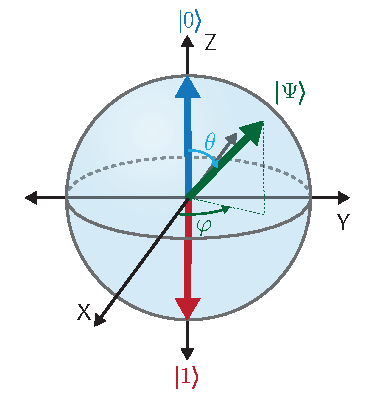
\includegraphics[width=0.5\linewidth]{BlochSphere}
  \caption[The Bloch sphere representation of a qubit]
  {The state of a qubit can be represented as vector on the surface of a unit sphere. In this description,
  the state is described by two angles: $\theta$ and $\psi$.}
  \label{fig:bloch}
\end{figure}

To see how this is true, it's helpful to rewrite the above state in spherical coordinates. First, let's
write $\alpha = r_0e^{-i\varphi_1}$ and $\beta = r_1e^{-i\varphi_2}$. The normalization condition is now
$r_0^2 + r_1^2 = 1$, from which we can make the replacement $r_0 = \cos(\theta/2)$ and $r_1 = \sin(\theta/2)$.
We can also factor out the phase $\varphi_1$ to give:
\begin{equation}
\ket{\psi} = e^{-i\varphi_1}\left(
    \cos\left(\frac{\theta}{2}\right)\ket{0} + e^{-i(\varphi_2 - \varphi_1)}\sin\left(\frac{\theta}{2}\right)\ket{1}
  \right)
\end{equation}
The term $e^{-i\varphi_1}$ is called a global phase factor, and is equivalent to a multiplication by a unit vector,
which it's easy to see makes no difference to the probabilities of any measurement (a fact that will continue to be
true even when we add more qubits). Another way of saying this is that the important information is encoded in
the relative phase between states. So, let's make the replacement $\phi = \varphi_2 - \varphi_1$ and ignore
the global phase factor, which gives us the state:
\begin{equation}
  \ket{\psi} = \cos\left(\frac{\theta}{2}\right)\ket{0} + e^{-i\phi}\sin\left(\frac{\theta}{2}\right)\ket{1}
\end{equation}
This representation is shown visially in Fig.~\ref{fig:bloch} and is called the Bloch sphere representation
of a qubit\footnote{For mathematicians, this is a description of the qubit in Complex Projective Space}.

Given this description, we can now start to think about what operations on a single qubit might look like.
While on a single bit, the only non-trivial operation we can perform is a flip ($0 \rightarrow 1$ and $1 \rightarrow 0$),
on a qubit we have a whole host of operations that we can perform. The only limits we put on ourselves is that these operations
must leave us on the surface of the Bloch sphere. In other words, after applying an operation, we must still
have a normalized state. From the Bloch representation, you may have already guessed that this means we
can only perform rotations.

Switching back to the 2D vector representation of a qubit, then it is also clear that these operations
must correspond to $2\times2$ matrices. The act of performing an operation corresponds to multiplying
the qubit state by one of these matrices. To ensure that the length of the qubit vector $\ket{\psi}$
remains one at all times, the matrices we can use on our qubit must be unitary. That is, given the matrix $\boldsymbol{M}$,
its complex conjugate transpose $\boldsymbol{M}^\dagger = (\boldsymbol{M^{*}})^\mathrm{T}$ times itself must be equal to
the identity matrix: $\boldsymbol{M}^\dagger\boldsymbol{M} = \boldsymbol{I}$.

Let's define three unit rotation matrices as $\pi$ rotations around the $X, Y, Z$ axes. These have the symbols
$\sigma_X, \sigma_Y, \sigma_Z$ respectively, and are called the Pauli matrices.
They have the values:
\begin{align}
  \sigma_X = \svec{0&1\\1&0} && \sigma_Y = \svec{0&-i\\i&0} && \sigma_Z = \svec{1&0\\0&-1}
  \label{eq:pauli}
\end{align}

We can build up arbitrary rotations from these unit vectors by taking various powers of these vectors
and multiplying them together. For example to apply a $\pi/2$ rotation around the y-axis applied to the state $\ket{\psi}$
we would perform $\sqrt{\sigma_Y}\ket{\psi}$\footnote{For those familiar with the rotation operators,
this is more commonly written with a phase factor to make the solution purely real: $R_Y(\tfrac{\theta}{2})
= \exp(-i\pi/4)\sqrt{\sigma_Y}$}.
A $2\pi$ rotation around the x-axis would be $\sigma_X\sigma_X\ket{\psi}$. It is possible to generalize this
to arbitrary rotations, giving us the rotation operators \cite{Nielsen:rot}:
\begin{align}
  R_X(\theta) = e^{-i \theta X/2} = \cos\left(\frac{\theta}{2}\right)\boldsymbol{I} - i \sin\left(\frac{\theta}{2}\right)\sigma_X \\
  R_Y(\theta) = e^{-i \theta Y/2} = \cos\left(\frac{\theta}{2}\right)\boldsymbol{I} - i \sin\left(\frac{\theta}{2}\right)\sigma_Y \\
  R_Z(\theta) = e^{-i \theta Z/2} = \cos\left(\frac{\theta}{2}\right)\boldsymbol{I} - i \sin\left(\frac{\theta}{2}\right)\sigma_Z
\end{align}
These three rotations (and often a global phase factor to simplify our result) are sufficient to express
any single qubit operation. For completeness, we can also define some other gates that often come up in
the context of quantum computation:
\begin{alignat}{4}
    H &=& \frac{1}{\sqrt{2}}\svec{1&1\\1&-1} &=& \, e^{\tfrac{i\pi}{2}} R_Y\left(\frac{\pi}{2}\right) R_Z(\pi) \, &=& \frac{\sigma_X+\sigma_Z}{\sqrt{2}} \\
    T &=& \svec{1&0\\0&e^{\tfrac{i\pi}{4}}}  &=& \, e^{\tfrac{i\pi}{8}} R_Z\left(\frac{\pi}{4}\right)          \, &=& \sqrt[4]{\sigma_Z} \\
    S &=& \svec{1&0\\0&i}                    &=& \, e^{\frac{i \pi}{4}} R_Z\left(\frac{\pi}{2}\right)          \, &=& \sqrt{\sigma_Z}
\end{alignat}
These are the Hadamard gate, the T gate (or $\pi/8$ gate)\footnote{The $T$-gate is often
referred to as the $\pi/8$ gate, even though it represents a $\pi/4$ rotation, a name that is derived from
the phase factor for historical reasons.} and the phase gate respectively.
As is typical, phase factors are usually dropped (something I did not do in the above), hence it is
common to see variations of these equations in the literature.

As a final example, let's take a detailed look at where interfering probabilities lead to a thoroughly
non-classical result. To start with, let's define two additional states:
\begin{align}
  \ket{+} = \frac{\ket{0} + \ket{1}}{\sqrt{2}} && \ket{-} = \frac{\ket{0} - \ket{1}}{\sqrt{2}}
\end{align}
We can get these states by starting from $\ket{0}$ and rotating $\pi/2$ or $-\pi/2$ around the Y-axis. You can
confirm that they are properly normalized, and that if we were to measure each state, the
probabilities of measuring a $\ket{0}$ or a $\ket{1}$ are equal for both states: $\mathrm{P}\left(\ket{0}\right) =
\mathrm{P}\left(\ket{1}\right) = 0.5$. So a direct measurement would be unable to distinguish these two states.
However, if we were to apply the Hadamard gate to each of those two states, we surprisingly end up with two
different outputs:
\begin{align}
  H\ket{+} = \ket{0} && H\ket{-} = \ket{1}
\end{align}
In this case, the complex probability amplitudes can interfere with each other causing the two states to
become distinguishable, something that a classical bit could not replicate. What you see is what you get.

\subsection{Multi-Qubit States (Qubit Registers)}
The next additional computational resource that quantum physics gives us is \textbf{entanglement}. This
resource rears its head when we try to combine multiple qubits into a register. Formally,
we can define entanglement as a correlation between the states of qubits after they have interacted
with each other. Due to this correlation, the state of a qubit that has been entangled with its partner
can no longer be described independently, the states of the two qubits become linked. Perhaps the easiest
way to grok the consequences of this is to give an example of how this correlation might play out.

Let's start with two qubits, one of which starts in the $\ket{+}$ state, and the other which starts in
the $\ket{0}$ state. If we were to apply a gate that flips the state of the second qubit if the state of
the first qubit is $\ket{1}$, then we might expect to end up with something like $\ket{+}$ in the second
qubit. If we measure the first qubit and get the result $\ket{0}$, the state of the second qubit must also
be zero, so the state of the second qubit can't have been described by $\ket{+}$. The state of the two
qubits is correlated and depend on each other. The operation we described above is called the
controlled-NOT ($CNOT$) gate, and creates a state that looks like:
\begin{equation}
  \ket{\psi} = \frac{\ket{00} + \ket{11}}{\sqrt{2}}
\end{equation}
To describe a generalized two-qubit state, we must give coefficients to each possible state the qubits
can take:
\begin{equation}
  \ket{\psi} = \alpha\ket{00} + \beta\ket{01} + \gamma\ket{10} + \delta\ket{11} =
    \svec{\alpha\\\beta\\\gamma\\\delta}
\end{equation}
So to combine two qubits together, we cannot just list the states of the two qubits one after another.
They are described by the tensor product of the two individual states: $\ket{\psi} = \ket{\psi_1}\otimes\ket{\psi_2}$.
For a three-qubit register, the total number of states we must give coefficients to is 8. For a $N$ qubit
register, the total number of coefficients is $2^N$. Note the distinction between a classical register
and a quantum register, to describe a classical register, we can list the states of the individual
bits one after another, whereas the quantum register requires $2^N$ complex numbers to express fully.

Much like a single qubit, we require new matrices that can operate on quantum registers. As one
might expect, the size of these matrices is exponential in the number of qubits that we must operate on.
For example, on a two-qubit register, we require a $4 \times 4$ matrix to describe operations. The
$CNOT$-gate that we used above is defined as:
\begin{equation}
  CNOT = \svec{1&0&0&0\\0&1&0&0\\0&0&0&1\\0&0&1&0}
\end{equation}
Unfortunately, the potential presence of entanglement means applying single or two-qubit gates to a subset
of qubits in the register is no longer a matter of applying a $2 \times 2$ or $4 \times 4$ matrix, we must
construct a $2^N \times 2^N$ matrix and apply that to the full quantum register. This construction is achieved
by taking the Kronecker product of identity matrices and the matrix we want to apply. For example, to apply
a $\sigma_X$ gate to the 2nd qubit in a three-qubit register, we construct the operator as follows:
\begin{equation}
  \sigma_{X,2} = \boldsymbol{I} \otimes \sigma_X \otimes \boldsymbol{I}
\end{equation}

The consequences of the twin effects of superposition and entanglement lead to the extra computational
power of a quantum computer, while also hinting at the difficulty of writing quantum algorithms. As we
can prepare arbitrary superposition states, we can encode an exponentially large
state into a quantum register, for example representing every number between 0 and $2^N-1$ in a $N$ qubit
register, and operate on all of these states in parallel. However, once we measure the register, we end up
with only one of the possible states in the register (i.e. the state collapses), and the quantum information
that was prepared in the state is lost. Quantum algorithms must, therefore, have three properties to be useful:
\begin{enumerate}
  \item An efficient way of preparing a state. If we want to perform computations on a quantum register
    storing $2^N$ values, we lose any exponential speedup if we need to load each of these values one-by-one.
    For example, Shor's algorithm relies on being able to prepare an equal superposition of all states
    in the register with $N$ single qubit gates \cite{PhysRevA.54.1034}.
  \item Creation of a large entangled state. Without entanglement, a quantum algorithm can be efficiently
    simulated on a classical computer. We don't know quite how to quantuntify the role that entanglement plays in computation,
    however, without using it, we know that quantum computers lose their advantage \cite{doi:10.1098/rspa.2002.1097}.
  \item A way of whittling down the quantum state to make the "answer" the likely outcome of any readout.
    Since coefficients in a quantum register represent probability amplitudes that measurement will yield
    a given outcome, we can get at most $N$ bits of data per measurement \cite{651037}, as our register
    immediately collapses into one state upon measurement. To get another value out of the register,
    we must repeat the whole computation, including loading the state.
\end{enumerate}

\subsection{Noise}

\begin{figure}
  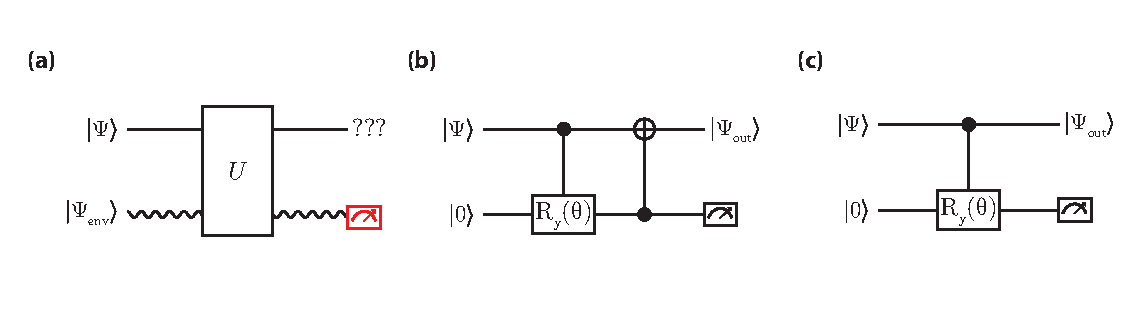
\includegraphics[width=\linewidth]{Noise}
  \caption[Noise affecting pure states]
  {(a) We can think of noise as uncontrolled interactions with an environment. However since we can't measure
  information that is transferred into the environment, we end up with an incomplete representation of our qubit.
  In order to represent this state, with some of its information lost, we must describe the state with a density
  matrix representation. (b) A simple model for relaxation, where we represent the probability of a decay $\gamma$
  in the rotation angle $\sin^2(\theta/2) = \gamma$. Each time this gate is applied, we end up more likely to be in
  the $\ket{1}$ state. (c) A simple model for dephasing, where the phase $\theta$ is a random variable. This type
  of quantum noise has no classical analog, but causes a loss of information about the relative phase between $\ket{0}$
  and $\ket{1}$.}
  \label{fig:noise}
\end{figure}

Up to this point we have assumed that there are no noise sources or sources of information loss in our
qubit implementations. Unfortunately, reality is not so kind, and as has been discussed before, it is the
fragility of a quantum state that remains the main challenge of implementing a large scale quantum computing,
an effect called~\textbf{decoherence}. Equivalently, we can describe this effect as uncontrolled coupling to the environment, either through
energy loss or uncontrolled rotations, which leads to loss of information from our quantum computer, as shown schematically
in Fig.~\ref{fig:noise} (a), where we see a qubit $\ket{\Psi}$ interact with the environment $\ket{\Psi_{\textrm{env}}}$.
As we are unable to make a good projective measurement of the environment, the output
state after the unitary interaction $U$ with the environment cannot be well described in the vector notation we have been using
this far, and some information about the state is irrevocably lost. The challenge of including
these sources of noise into our view of quantum computing is to figure out how to model the uncontrolled
environment\footnote{Or, we could replace the environment with something we CAN control and measure, an approach attempted
in \cite{s41586-019-1287-z}.}.
The primary way to describe such an interaction is to switch to a density matrix representation of our state, which allows us
to describe a subsystem of a composite quantum system, i.e. to ignore the portion of the state lost to the environment.
Indeed, this is the most complete way to describe noise processes and information loss of our state, however rather
than introduce a more powerful and complex, but otherwise equivalent, description of quantum mechanics, we can instead model
noise processes as interactions with a controlled and known environment, such as another qubit, as in Figs.~\ref{fig:noise} (b) and (c).
We can categorize interactions of our qubits into two general classes: relaxation (sometimes called amplitude
damping), and dephasing (sometimes called phase damping), which collectively lead to decoherence.

The first class of error, \textbf{relaxation}, causes our population to decay towards the ground state $\ket{0}$ each time it is
applied with probability $\gamma$. We can think about this sort of process as a loss of energy from the qubit system, and
in a way is analogous to classical relaxation, for example of an pendulum which gradually loses energy to the environment
or an atom in an excited state that decays. An equivalent circuit for such a process into a controlled environment (a second qubit) is
shown in Fig~\ref{fig:noise} (b), where the portion of the state in $\ket{1}$ undergoes a gradual rotation $R_{y}(\theta)$
towards the $\ket{0}$ state, where the phase $\theta$ is chosen to represent the probability of a relaxation event:
$\sin^2(\theta/2) = \gamma$. We represent the permanent loss of the information as a projetive measurement made on the
second qubit. This error is commonly quoted in literature as a $T_1$ time, where $T_1$ is a time constant
that gives us the rate at which a state will decay towards the ground state. Thus the probability of a relaxation event occuring
after time $t$ is given by:
\begin{equation}
  P(\ket{1} \rightarrow \ket{0}, t) = 1 - e^{-t/T_1}
\end{equation}

The second form of error, \textbf{dephasing}, is one that does NOT have a classical analog, and represents randomization of the phase between
states in the qubit or qubit register. Understanding the effect of this sort of noise is harder than for relaxation since there is no
classical analog, however if we permit ourselves a Bloch sphere representation of a qubit, we can visualize it
as a randomization of the $\varphi$ angle. An equivalent circuit, again using a second qubit to simulate the
environment is shown in fig.~\ref{fig:noise} (c). We represent an irretrievable loss of information to the
environment as a projective measurement on the second qubit. This error rate is commonly quoted as the $T_2$ time,
the rate that phase information is lost to the environment. In the case of a single qubit evolving under completely uncorrelated
(Markovian) noise, this would be the end of the story, however in most systems, we also define a $T_2^*$, an ensemble
dephasing time. In the case of single qubits that evolve under quasi-static noise
\footnote{Quasi-static noise is noise that is approximately constant over the timescale of qubit operations. More formally,
we can define it as non-Markovian noise, that is there is some correlation in the noise that we can learn and correct
by appropriate application of dynamical decoupling.} or multi-qubit systems that operate
under an inhomogeneous background, we can use correlations in the noise or the static nature of the inhomogeneous background
to "rephase" our qubits \cite{PhysRev.80.580,dynamic-decoupling-biercuk}. We can think of this effect as coming from the
fact that the phase evolves at a predictable rate over the timescale of operations, such that by applying an appropriate sequence
of gates, we can unroll whatever phase was accumulated.  In this case, the $T_2$ time becomes the dephasing time after
application of rephasing gates, while $T_2^*$ is the ensemble dephasing time, assuming measurement over a longer timescale
than the correlation time and without correcting for inhomogeneities.

\section{Making Qubits in Semiconductors}
\label{sec:qcinsm}
% TODO: Add references to each of the types of qubits
Having described the basic ideas of quantum computing, our next challenge is to find a physical system that
can implement the operations that we discussed above. This problem can be distilled to that
of finding a quantum two-level system conforming to a set of criteria that were first laid out by David
DiVincenzo, criteria that are widely considered to be the standard checklist for any qubit system \cite{divincenzo_crit}. They are:
\begin{enumerate}
  \item A scalable physical system with well-characterized qubits.
  \item The ability to initialize a fiducial qubit state, such that the state of the system is known prior
    to any quantum operations.
  \item Decoherence times in the qubit subspace that greatly exceed the gate operation time.
  \item A universal set of quantum gates.
  \item The ability to perform measurements on individual qubits.
\end{enumerate}
Although these criteria set out some requirements for useful qubits, they are certainly not so prescriptive
that there is a dearth of systems that could fulfil them. It is in this context that ion-trap qubits, photonic qubits,
NMR based qubits, superconducting qubits and semiconductor-based qubits are being investigated as the base of a quantum computer, each satisfying the
criteria to varying degrees. I will focus on semiconductor-based qubits for the remainder of this thesis. This type
of qubit has the potential to utilize the extraordinary processing capabilities of modern semiconductor manufacturing.
Despite narrowing the focus to semiconductor systems, there are still many
choices of two-level subspace we could use. I will not attempt to cover all the variations
of qubit that exist; rather I will focus specifically on two general designs, quantum dots and Majorana zero modes,
which in many ways share similar control and readout. As such the discussion of physics in this section will
largely be confined to III-V materials, although I will point out that as my thesis is aimed at the general
problem of architecting a quantum computer, many of the results presented may are extensible to quantum
computers beyond spins and Majoranas. Before we begin a detailed discussion of qubits in semiconductors, let's first take a look
at the physics that underlie most of these implementations; the 2-dimensional electron gas (2DEG).

\subsection{The 2-Dimensional Electron Gas}
\label{sec:2deg}
The 2-dimensional electron gas (2DEG) is the foundation for many of the experiments and qubit-realizations to follow and
is a confinement of electrons in a semiconductor to a single plane. To fully
appreciate what this means, we first have to discuss what it means to confine an electron in one of the three dimensions.
How do we make a confining potential that can create a sheet of electrons a single electron thick? How narrow
would such a potential have to be? To answer this question, we must look at the solutions
to Schrödinger's equation in a semiconductor. These solutions will give us the distribution of the electron wavefunction, and
an idea of its "size". The following introduction is based on material taken from \cite{delftbook, ihnbook, Ashcroft}.

\begin{figure}
  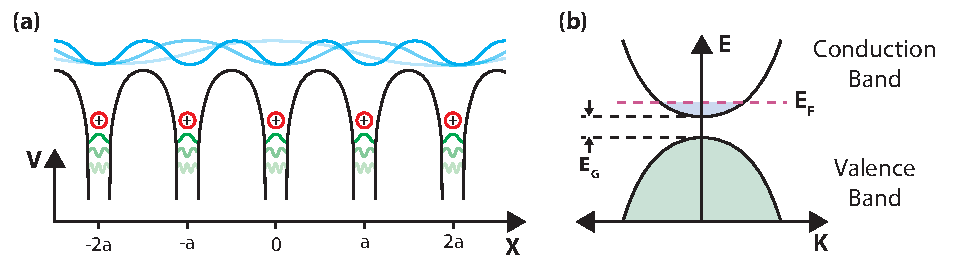
\includegraphics[width=0.9\linewidth]{BlochWaves}
  \caption[Bloch waves on a regular lattice]
  {(a) Given a periodic lattice that creates a set of potential wells, the valid solutions for unbound
   electrons (conduction band) are plane waves with a wave vector proportional to the lattice spacing $a$,
   while solutions for bound electrons (valence band) are proportional to the strength of the potential created
   by the constituent elements of the lattice. (b) Assuming there are no electron-electron interactions,
   and the lattice may be treated as a small peturbation to plane wave solutions (the nearly-free electron model),
   the band structure will be parabolic, with a band gap $E_G$ between the valence and conduction bands, where there are
   available states. Electron states are filled to the Fermi energy ($E_\textrm{F}$).}
  \label{fig:blochwaves}
\end{figure}

In a crystalline material, such as a metal or a semiconductor lattice, we can think
about electrons as travelling through a periodic potential, caused by the periodic spacing of nuclei in the lattice, as
is shown in Fig.~\ref{fig:blochwaves}~(a) for a 1D lattice. There will be two sets of solutions; one for electrons
that are bound around nuclei which will form the valence band and one for free electrons which
will form the conduction band. The gap between these two solutions forms a band gap of size $(E_G)$, a range
of energies for which there are no available states. As we are looking at the 2DEG, let's focus on free electron solutions for now.
These solutions will take the form of Bloch waves, expressed as a function of lattice position $r$ and wave-vector $k$:
\begin{equation}
  \psi_{\vec{k}}(\vec{r}) = e^{i\vec{k} \cdot \vec{r}}u_k(\vec{r})
\end{equation}
where $u_k$ is a periodic function with the same periodicity as the crystal lattice and $e^{i\vec{k} \cdot \vec{r}}$ are
the general form of plane waves. What this equation effectively means is that if we are able to solve around boundary conditions for
a single unit cell, we can extract a band structure for the entire lattice.

Electrons in this system begin to fill the available states from the lowest energy up, obeying the Pauli exclusion principle which limits
each available state to two electrons with opposite spins. For conduction band electrons in uniform crystals, we can make
two additional assumptions that aid in the interpretation of the solutions to the Bloch equation. First, let's assume that
there are no electron-electron interactions. Although this assumption may at first be unintuitive, it appears
to be sufficient to describe much of the physics that follows. Second, we assume that the potential due to the
lattice is screened by valence band electrons, and can be treated as a small perturbation to a free electron. Solving
this model leads to bands which are similar to free electron plane waves up to the edge of the Brillouin zone, i.e.
up to the top of the band. In the conduction band of a semiconductor, we deal with largely empty bands, as such
the dispersion relation, i.e. the energy of electrons as a function of the wave-vector, can be approximated as that of free electrons:
\begin{equation}
  E(\vec{k}) = \frac{\hbar^2 |\vec{k}|^2}{2m^*}
  \label{eqn:3ddisp}
\end{equation}
where $\vec{k}$ is the electron wave-vector and $m^*$ is the effective electron mass that derives from the peturbation of the lattice.
The effective electron mass in this instance is a scaling factor on the increase in energy as wave-vector changes and is
defined as the curvature of the conduction or valence band of the semiconductor:
\begin{equation}
  m^* = \hbar^2 \left(\diff[2]{E}{k}\right)^{-1}
\end{equation}
Intuitively we can think of it as describing a change in momentum for a given energy "kick". For a parabolic and isotropic
band, such as for the bottom of the conduction band in a III-V semiconductor, its value is constant, however
the form of the effective mass will be more complex for materials that have directional dependences (such as Si),
or more complex band structures such as graphene. From Eqn.~\ref{eqn:3ddisp}, we can also give the
formal definition for the Fermi energy. The \textbf{Fermi energy} ($E_F$) is the energy of the highest filled electron state
at zero temperature. This situation is represented schematically in Fig.~\ref{fig:blochwaves}~(b) for a single dimension.
In 3D, the Fermi energy forms the surface of a sphere in momentum space delineating the region where electron states are filled,
which we call the Fermi surface. Finally, we can define the \textbf{Fermi wavelength} $\lambda_F$ of an electron at the Fermi
surface, effectively the size of an electron in our semiconductor. Using $k = 2\pi/\lambda$ we find:
\begin{equation}
  \lambda_F = \frac{h}{\sqrt{2m^*E_F}}
\end{equation}

\begin{table}
  \centering
  \begin{tabular}{|l|l|l|}
   \hline
   Crystal & Lattice Constant (\si{\angstrom}) & Electron Effective Mass$(m^*/m_e)$ \\
   \hline
   Si & 5.43 & - \\
   Ge & 5.658 & - \\
   GaAs & 5.65 & 0.066 \\
   InAs & 6.06 & 0.026 \\
   InSb & 6.48 & 0.015 \\
   \hline
  \end{tabular}
  \caption[Properties of some common semiconductors]
  {Lattice constants and effective electron masses for some common semiconductors. For Si and Ge semiconductors, which are
  indirect band gap semiconductors, the effective mass for electrons is not trivial and will vary based
  on direction and valley state, hence values are not given above. Values are taken from \cite{Kittel2004,InSbParam}.}
  \label{tab:semiprop}
\end{table}

If we wish to confine electrons in a given dimension, the Fermi wavelength gives us the length-scale on which we must form
our confining potential. For metals, the large number of free electrons means the Fermi energy is large, and as such we end up with a
Fermi wavelength on the order of a few Ångström (where $\SI{1}{\angstrom} = \SI{1e-10}{\meter}$). In semiconductors, as
the number of free electrons, and hence the Fermi energy, is set by the doping and is generally small, the Fermi
wavelength can be on the order of a few 10s of nanometers. Parameters for some common semiconductors are given
in Table~\ref{tab:semiprop}. Given these values, if we can make a potential well with a width $W$ that's on
the order of the Fermi wavelength, we can confine electrons to a few subbands. The next question is: how
do we create a narrow quantum well?

\begin{figure}
  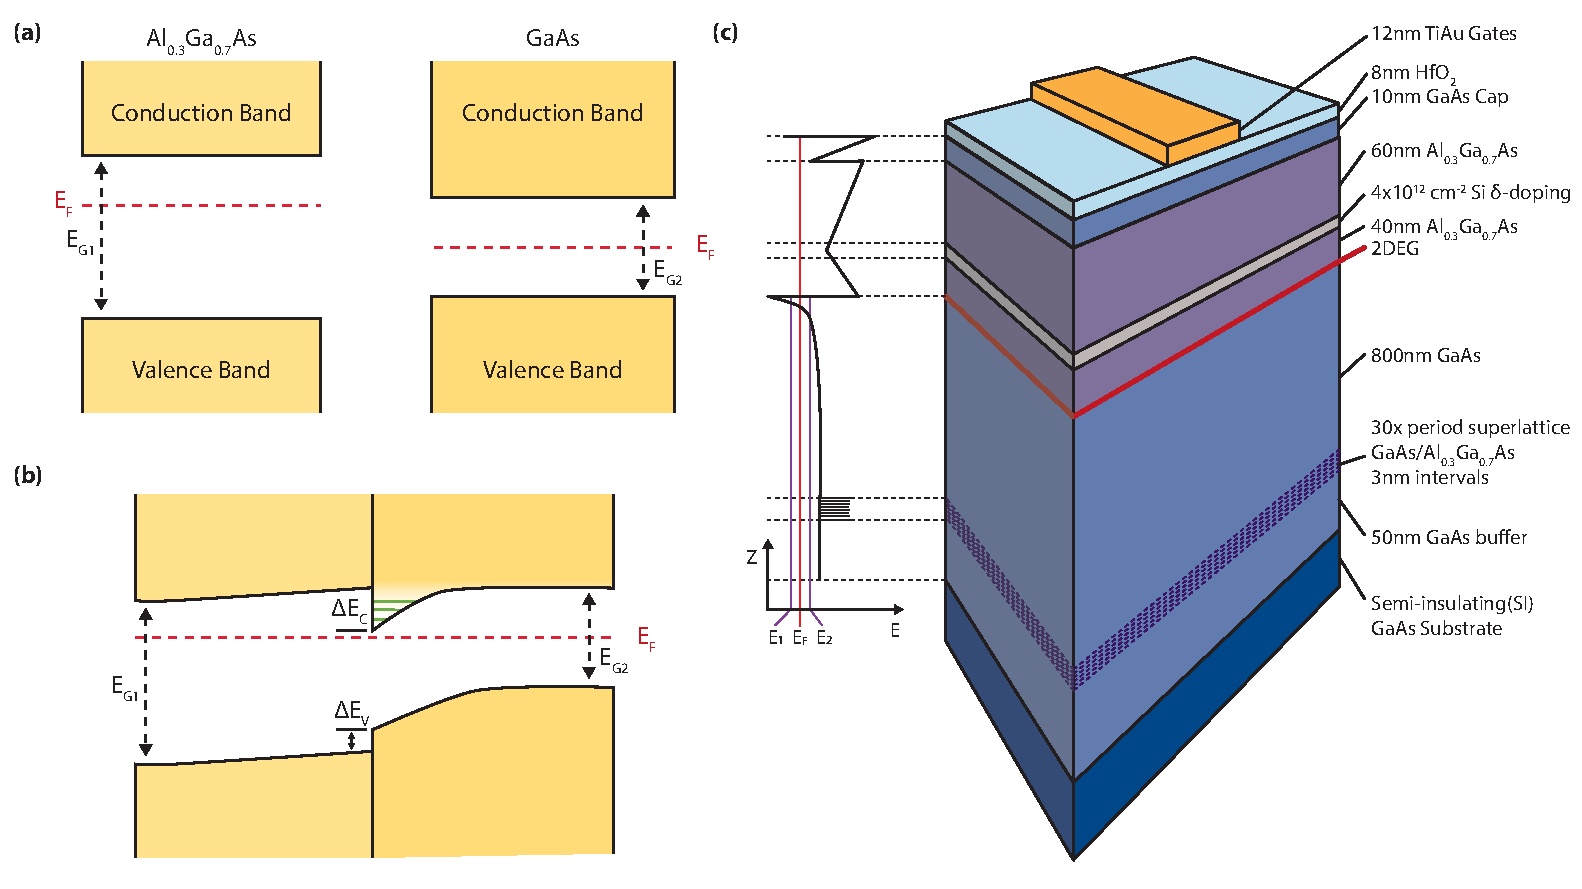
\includegraphics[width=1\linewidth]{GaAs}
  \caption[Band bending in a straddling type heterojunction, and the GaAs/AlGaAs heterostructure]
  {\label{fig:heterostructure}(a) Shows a straddling type heterojunction between \ce{Al_{0.3}Ga_{0.7}As} and GaAs with two
  differing bandgaps $E_{G1}$ and $E_{G2}$, where the smaller gap ($E_{G2}$) is fully enclosed in the larger gap $E_{G1}$.
  (b) When the two semiconductors are equalized, their bands bend near the heterojunction to ensure a continuous Fermi energy.
  Far from the junction, the unmodified band structure is restored. (c) The layer stack of a GaAs/(Al,Ga)As heterostructure,
  with TiAu surface gates that can locally modify the density of the 2DEG.}
\end{figure}

The answer is to create a heterojunction; an interface between two dissimilar semiconductors with different band-gaps.
The simplest type of heterojunction we can form is a straddling (type I) junction, where one semiconductor has a smaller band-gap
that is contained within the band gap of the other, a situation that is represented schematically in Fig.~\ref{fig:heterostructure} (a).
In the case that the Fermi levels of the two semiconductors are unequal, electrons tunnel through the junction to align
their levels, leading to band bending at the interface. Careful choice of semiconductors can cause a well to appear at the interface,
where the width of the well can be designed to be on the order of the Fermi wavelength in the semiconductor. GaAs and (Al,Ga)As are
an ideal choice for this type of heterojunction as they are almost perfectly lattice matched (their lattice constants differ by 0.14\%),
while also forming a straddling-gap heterojunction. The gap in GaAs is $E_{G1} = \SI{1.424}{\electronvolt}$ and the gap in
\ce{Al_{x}Ga_{1-x}As} can be continuously varied by
changing the ratio of Al and Ga in the semiconductor, taking the value $E_{G2} = 1.424 + 1.225x$ \si{\electronvolt}.
Furthermore, between $x = 0$ and $x = 0.44$, the bandgap is direct and ratio of the step in the conductance
band ($\Delta E_C$) to the step in valence band ($\Delta E_V$) is a constant: $\Delta E_C/\Delta E_V = 1.5$\cite{adachi1993properties}
[see steps in Fig.~\ref{fig:heterostructure}~(b)], allowing the depth of the well to be easily varied.
Finally, by doping the semiconductor with Si, we can move the Fermi energy up to populate a single subband, leading to a
2-dimensional plane of electrons, where there is only a single wave-vector in the Z direction ($k_z$) that electrons can take. As long
as the electron temperature is far below the energy gap of the subbands, only this subband will be populated.

The structure of a typical GaAs/\ce{Al_{0.3}Ga_{0.7}As} heterostructure is shown in Fig.~\ref{fig:heterostructure}~(c). Such structures
are normally grown by molecular-beam epitaxy (MBE) which allows atomically smooth layers to be grown a single monolayer
at a time. We start with a semi-insulating GaAs substrate, over which a large buffer is grown.
Repeated thin layers of GaAs/\ce{Al_{0.3}Ga_{0.7}As} are grown to reduce the dislocation density
and create a continuous, smooth single crystal at the heterojunction, and to trap impurities which may percolate upwards
during the annealing stage of the growth. The red line represents the 2DEG itself on the schematic,
followed by a region of Si $\delta$-doping, used to pin the Fermi level in the substrate, and
a \SI{10}{\nano\meter} GaAs cap to protect against oxidation. During processing, a protective oxide barrier
(either \ce{HfO2} or \ce{Al2O3}) is grown, followed by surface gates which allow the density of states to be locally modified, or even depleted,
to define structures in the 2DEG. The oxide layer, apart from serving as a passivation barrier, is also necessary to
prevent tunnelling of electrons from the surface gates into the donor layer, where the movement of electrons is known to be a significant
source of charge noise \cite{PhysRevB.72.115331, PhysRevApplied.9.034008}.

Having confined electrons into 2-dimensions, we can now redefine several of the parameters that we had above. First, our
dispersion relation becomes that of free electrons in two-dimensions:
\begin{align}
  E(\vec{k}) = \frac{\hbar^2 |\vec{k}|^2}{2m^*} && |\vec{k}|^2 = k_x^2 + k_y^2
  \label{eq:k2d}
\end{align}

We can also define the density of states (DOS) in 2-dimensions as the number of states $n(E)$ per unit energy $(E)$:
\begin{equation}
  \rho_{2D} = \diff{n(E)}{E}
  \label{eq:raw2dden}
\end{equation}

For free electrons in 2D, the states fill an area in momentum-space up to k-vector $k$:
\begin{equation}
  A = \pi k^2 = \frac{2 \pi m^* E}{\hbar^2}
\end{equation}
where we've substituted equation~\ref{eq:k2d} for $k$. The spacing of states in a crystal of size $L \times L$ is given
by $\pi^2/4 L^2$, so for a unit area, the area of a single state is $A_{\textrm{single}} = \pi^2/4$. Putting this together,
the number of states up to energy $E$ is therefore:
\begin{equation}
  n(E) = g_s g_v \frac{A}{A_{\textrm{single}}} = g_s g_v \frac{m^* E}{2 \pi \hbar^2}
\end{equation}
and giving a density of states:
\begin{equation}
  \rho_{2D} = g_s g_v \frac{m}{2 \pi \hbar^2}
  \label{eq:2dden}
\end{equation}
where $g_s$ is the \textbf{spin degeneracy} (almost always 2), and $g_v$ is the \textbf{valley degeneracy} (1 for III-V semiconductors, 3 for Si).
Importantly we note that the density of states is independent of energy, a situation which is unique to 2-dimensions.
Finally, we redefine the Fermi energy, wave-vector and wavelength in terms of the total electron density ($n_s$), which give the following equations:
\begin{align}
  E_F = \frac{n_s}{\rho_{2D}} = \frac{2 \pi \hbar^2 n_s}{m^* g_s g_v} &&
  k_F = \sqrt{\frac{4 \pi n_s}{g_v g_s}} &&
  \lambda_F = \sqrt{\frac{\pi g_s g_v}{n_s}}
\end{align}

Having detailed the formation of 2DEGs, we must now consider the factors that will affect their quality for
experimental purposes. Broadly, the two most important effects that will affect the quality of the
2DEG are temperature and scattering. First, the main effect of temperature will be to create a distribution of filled states around the Fermi energy, rather
than a sharp cut-off as we had previously assumed. This distribution is called the Fermi-Dirac distribution and takes the form:
\begin{equation}
  f(E - E_F) = \left[1 + \exp\left(\frac{E - E_F}{k_B T}\right)\right]^{-1}
\end{equation}
This thermal population places an additional constraint on 2DEG formation, namely that the thermal energy $k_B T$ should be much less than the
2D subband spacing, a requirement that is easily met for most heterostructures below a few Kelvin. Second, we account for the
effect of scattering, which we capture in the form of a length that an electron can travel before scattering. Depending on the scattering
mechanism this can either be inelastic, normally due to scattering off phonons (thermal scattering), or elastic, normally due to
scattering off lattice defects or impurities. Therefore we define two length scales, $l_\psi$ being the inelastic scattering length,
which gives us the length scale over which total kinetic energy and momentum are conserved, and $l_e$ being the elastic scattering
length, which gives the length of time an electron will travel before any collision. From this, we can also define the momentum relaxation time, the
amount of time between electron collisions, given by $\tau = l_e/v_F$.

In general, we are more interested in the effect of scattering on conductivity, an easily measured bulk property of
the semiconductor. We can reframe the scattering time into a conductivity by considering the motion of an electron
through a lattice. Let's define a quantity called the drift velocity $v_d$ as the average speed an electron moves through
the lattice under an accelerating field $E$. Then, by Newton's second law:
\begin{equation}
  eE = \frac{m^* v_d}{\tau}
\end{equation}
If we rearrange for $v_d$ we find:
\begin{align}
  && v_d = \mu E && \left(\textrm{where~} \mu = \frac{e \tau}{m^*}\right)
  \label{eq:driftv}
\end{align}
where $\mu$ is a quantity called mobility, with units \si{\square\centi\meter\per\volt\per\second}.
To find the conductivity, we remember the definition for current
density, which will be given by the number of electrons that pass an area per second:
\begin{equation}
  J = n_s e v_d
  \label{eq:currden}
\end{equation}
This is combined with the definition of conductivity, which is simply the current density per electric field, $\sigma = J/E$. From here,
we find the equation for conductivity in terms of electron density and mobility to be:
\begin{equation}
  \sigma = n_s e \mu
  \label{eq:cond}
\end{equation}
We will revisit these equations, adding quantum corrections where necessary, and expand on scattering mechanisms within a
2DEG in Section~\ref{sec:char}.

At this point, our discussion splits into two streams.
The first deals with the formation of quantum dots, structures with tight confinement in all three dimensions,
and is covered in Section~\ref{sec:qd}. The second deals with the characterization of 2DEGs, extracting
the mobility, density, strength of the spin-orbit interaction, via weak (anti-)localization measurements and the quantum
Hall effect, and is covered in Section~\ref{sec:char}. Both of these are crucially important for building a variety of
qubits in semiconductors, and many of the advances in both spin qubits and topological qubits stem
from improvements in materials science that have led to higher quality 2DEGs and the availability of exotic material systems.

\subsection{Quantum Dots}
\label{sec:qd}
Let's now consider the question of how we might use the 2DEG to form a qubit. This can occur in many different
ways, for example through the creation of superconducting Josephson junctions with a 2DEG to tune the Josephson
energy \cite{karl-gatemon} or in Majorana zero modes \cite{PhysRevLett.119.136803}, formed using a 2DEG as a starting
point, a topic we shall explore in Section~\ref{sec:majo}. By far the most well studied 2DEG based qubit is the zero-dimensional
quantum dot, used to confine electrons using surface gates to define zero-dimensional "puddles" of electrons
\cite{RevModPhys.79.1217,RevModPhys.75.1}.
These puddles of electrons, which in a semiconductor have dimensions on the order of the Fermi wavelength $\lambda_F$,
creates a discrete spectrum of available states, a situation akin to having an atom with a set of orbital modes
defined in the middle of your 2DEG \cite{PhysRevLett.77.3613}. Before considering a quantum dot in a semiconductor, let's
start by looking at a small metal island, which will not have well resolved orbital modes but can still contain a discrete,
well defined, number of electrons.

\begin{figure}
  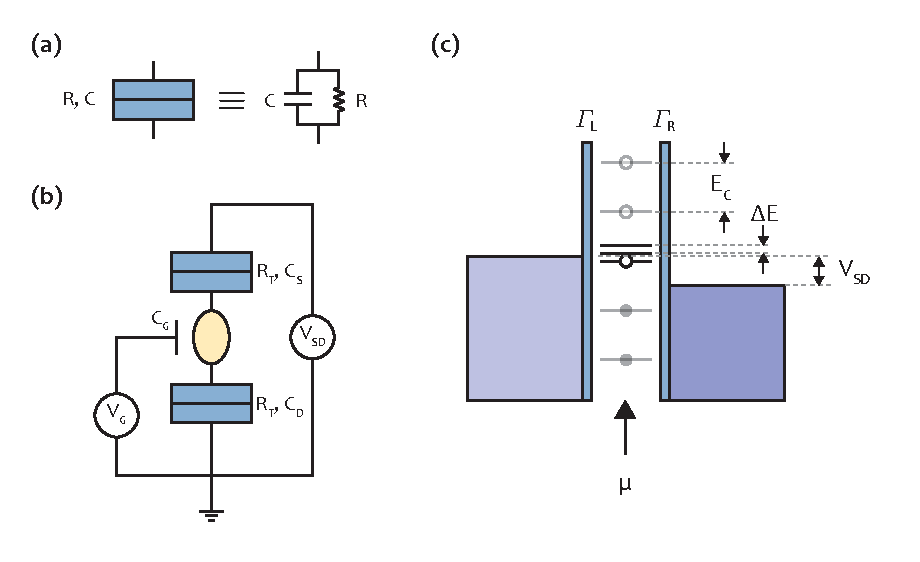
\includegraphics[width=0.8\linewidth]{Dot}
  \caption[Schematic of a single quantum dot]
  {\label{fig:QD}(a) We define a tunnel junction as a combination of a resistor and a capacitor in parallel
  since for a quantum dot the geometric capacitance of the junction is significant. (b) Equivalent circuit
  model of a quantum dot. The dot is connected to reservoirs by a source and drain tunnel junction, where
  we define the drain as ground. A voltage $V_SD$ may be applied across the quantum dot, which may cause current
  to flow. The levels of the quantum dot can be tuned by a gate voltage $V_G$ that is capacitively coupled to the
  quantum dot. (c) Schematic of a quantum dot showing a "ladder" of states, and orbital energy level. When a level
  falls within the source-drain bias window current may flow across the dot, otherwise current is blocked, an
  effect termed Coulomb blockade.}
\end{figure}

To understand how this is possible, we begin with the formula for the energy on a capacitor, the same one that
we initially give for a classical capacitor. This is given by: $E = Q^2/2C$. The energy to add a single extra electron
to this island is the \textbf{charging energy}:
\begin{equation}
  E_C = \frac{e^2}{2 C_{\Sigma}}
\end{equation}
where $C_\Sigma$ is the total capacitance to the dot. We then couple this island to two reservoirs, say a source
and a drain, both with resistance $R_t$. Realistically, these coupling resistances each add a capacitance term, which
we must consider in our $C_\Sigma$ term, as shown in Fig.~\ref{fig:QD} (a). We can also add a gate nearby that we can use to pull electrons on and off
the island. This situation is represented schematically in Fig.~\ref{fig:QD} (b). You might ask what differentiates
this system from a circuit I could make on my bench with three capacitors and two resistors. In other words, what are
the conditions for the number of electrons on the dot to be well defined? Firstly, we want the thermal energy
in the system to be much smaller than the charging energy; otherwise, we won't have a well-defined ground state:
\begin{equation}
  k_B T \ll E_C
\end{equation}
Next, we want to ensure that tunnelling occurs at a slow rate relative to the Heisenberg uncertainty relation
$\Delta E_C \Delta t \geq h/2$. If this condition is not met, dots can hop on and off the dot faster than we could resolve them.
The tunnelling time is given by $\tau = R_t C$, the time constant of the system. Combining $\tau$ and $E_C$,
we derive our second restriction:
\begin{equation}
  R_t \gg h/e^2
\end{equation}
This quantity $h/e^2$ is called the vonKlitzing constant, or the quantum or resistance, and will show up
throughout this thesis in several contexts; as the resistance of a 1D channel, the resistance of an edge
state in the quantum Hall and spin quantum Hall effect and the tunnelling rate through coupled Majorana zero modes,
and has the value $R_K = \SI{25812.807}{\ohm}$.

From here, we can define the total energy of the quantum dot with $N$ electrons. To do this, we will use a
semi-classical model called the constant-interaction model. This model defines the energy in terms of the background charge $N_0$, and
\footnote{We can think of the background charge $N_0$ as the quantized equivalent of the Fermi energy. It is equivalent
to $E_F = N_0^2 E_C$, and tells us how many electrons are in the dot at zero gate voltage.},
the voltage and the capacitance of the source, drain, and gate. At this point we can work in the limit of
a small-sized dot relative to the Fermi wavelength, and reintroduce the orbital energy levels $E_n(B)$. Here $E_n(B)$
is defined as the energy of the $n$-th orbital under a magnetic field B. This gives the equation for total energy of the quantum
dot as:
\begin{equation}
  U(N) = \frac{[-|e|(N-N_0) + C_SV_S + C_DV_D + C_GV_G]^2}{C_\Sigma} + \sum_{n=1}^{\left\lfloor\frac{N}{g_sg_v}\right\rfloor} E_n(B)
\end{equation}
Note that we've included the spin and valley degneracies in the filling of the orbital states of the quantum dot in
the summation of $E_n(B)$. We can also define the electrochemical potential $\mu(N)$ of the dot:
\begin{multline}
  \mu(N) \equiv U(N) - U(N-1) \\
    = \left(N - N_0 - \tfrac{1}{2}\right)E_C - \frac{E_C}{|e|}\left(C_SV_S + C_DV_D + C_GV_G\right) + E_{n}(B)
  \label{eqn:onemu}
\end{multline}
Note that we've assumed that we are tunnelling into the lowest unoccupied orbital energy level $E_n$. It is a reasonably
simple modification to Equation~\ref{eqn:onemu} to calculate the chemical potential of tunnelling into an excited orbital
state. The most important difference between the chemical potential $\mu$ and the energy $E$ is the linear dependence on gate voltage,
which allows us to draw a "ladder" of states where the gap between each state is a fixed value:
\begin{equation}
  E_{\textrm{add}}(N) = \mu(N+1) - \mu(N) = E_C + \Delta E_n
\end{equation}
This is depicted schematically in Fig.~\ref{fig:QD} (c). This equation also shows us that the electrochemical
potential of the dot can be swept linearly by varying the gate voltage.

\begin{figure}
  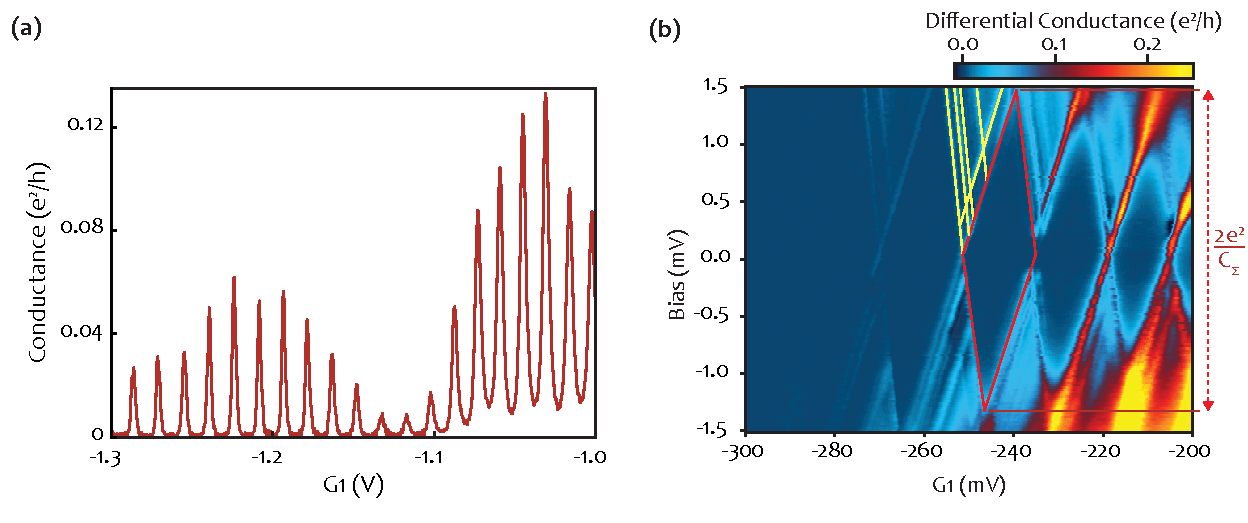
\includegraphics[width=1.0\linewidth]{CB}
  \caption[Coulomb blockade in a single quantum dot]
  {\label{fig:cbtrans}(a) Coulomb blockade through a single quantum dot. Current can only flow at points
  where the energy levels in the dot are in alignment with the reservoirs, which occurs as the gate voltage
  is swept. (b) Sweeping bias as well as the gate, we get diamond-like features as the levels move into
  and out of the bias window. The charging energy can be extracted by looking at the width of a diamond, as
  shown in red, and increases as the size of the dot is reduced by a more negative confining potential. We can
  also see excited states within each diamond, highlighted in yellow on a single diamond. These correspond to orbital
  modes within the quantum dot.
  }
\end{figure}

The next question we might ask is: how can we flow current through the dot. Current can only flow via the addition of an electron
from the source ($N \rightarrow N+1$) and the removal of an electron to the drain ($N+1 \rightarrow N$), which only occurs
when the electrochemical potential $\mu(N)$ falls within the source-drain window of the reservoirs for some N:
\begin{equation}
  E_F - \frac{|eV_{SD}|}{2} \leq \mu(N) \leq E_F + \frac{|eV_{SD}|}{2}
\end{equation}
This leads to a peaked conductance spectrum at low source-drain bias as a gate voltage is swept (as in Fig~\ref{fig:cbtrans} (a)), or
diamond-like regions of blocked conductance as source-drain bias is swept as a function of gate voltage (as in Fig~\ref{fig:cbtrans} (b)),
an effect termed Coulomb blockade. The spacing of Coulomb diamonds allows the extraction of charging energies and addition energies, as
well as the lever arm $\alpha$. This is the ratio of gate capacitance to total capacitance for each gate that is swept. The width of Coulomb
peaks reveals information about the temperature of the electrons, as high electron temperatures smear the population in
the source and drain reservoirs. I do not give a derivation of this effect here; however, we point the curious reader to \cite{grabert2013single},
and note that this is the method by which we extract electron temperatures in Section~\ref{sec:gooseberry}.

\subsubsection{Double Quantum Dots}
\begin{figure}
  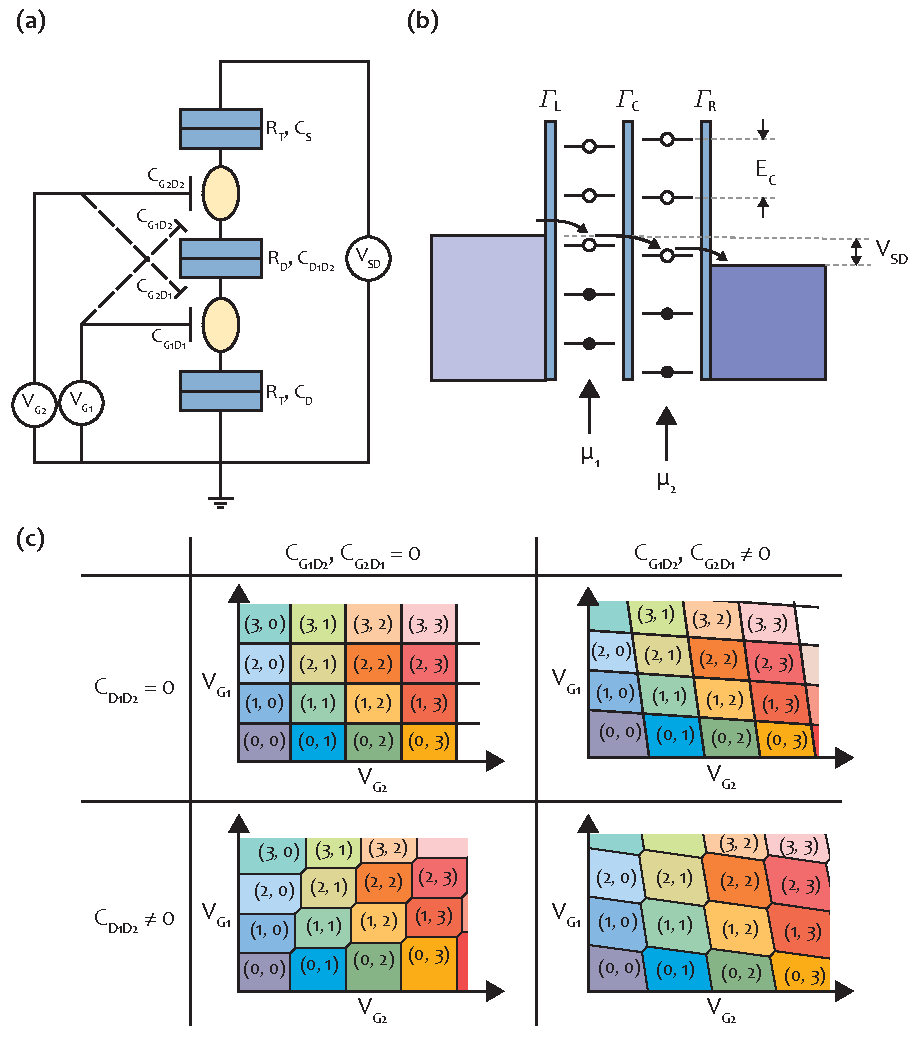
\includegraphics[width=1.0\linewidth]{DoubleDot}
  \caption[Schematic of a double quantum dot]
  {\label{fig:dqd}(a) Equivalent circuit model for a double quantum dot. The circuit is very similar to that of
  two single quantum dots in series, except that we must also account for cross capacitances between adjacent gates
  (the terms $C_{G1D2}$ and $C_{G2D1}$), as well as the contribution of the tunnel junction between the left and
  right dots (the term $R_D$ and $C_{D1D2}$). (b) Energy levels in a double quantum dot system. For current to flow
  through this circuit, there must be an available level in both the left and right quantum dots. (c) Here we map
  out the effect of cross capacitance and inter-dot capacitance on the charge stability diagrams of a double quantum
  dot system as $V_{G1}$ and $V_{G2}$ are varied. As each $V_{G1}$ ($V_{G2}$) becomes more positive, more dots are
  pulled onto the left (right) quantum dot. If gate capacitance is non-zero, the lines take on a slope. If inter-dot
  capacitance is non-zero, each stable configuration splits into a hexagonal cell. Note that these drawings do
  not include the effects of tunnelling between dots.}
\end{figure}

Before we move onto a discussion of how we might use these to form qubits, I will introduce the double quantum dot,
where we couple two single dots together. Much like we can consider a single quantum dot an
artificial atom, so too we can consider two quantum dots that allow tunnelling of electrons between each side as
an artificial molecule. The extension of the single quantum dot picture to a double quantum dot picture occurs by
adding a tunnel junction between the left and right dots, and adding a gate to control the
electrochemical potential of the second quantum dot, as shown in Fig.~\ref{fig:dqd} (a).
To completely model the effect of a double quantum dot, we must account for two additional sources of capacitance, first
a cross-capacitance between the left (right) gate and the right (left) quantum dot, and second the capacitance between
the left and right dot. Intuitively we can understand the capacitance between dots as a new electron on the left dot
shifting the energy and chemical potential of the right dot or vice-versa, leading to a shift in the locations of charge
transitions as electrons are pulled on and off each quantum dot. To characterize the effect of the two gates on a double
quantum dot, we can plot the ground state occupancy of the quantum dots as each of the gate voltages is swept, in a plot
called a charge stability diagram. A mockup of charge stability diagrams are shown in Fig.~\ref{fig:dqd} (c) as both interdot
capacitance and gate cross-capacitance are turned on and off. The occupancy of the double quantum dots is labelled
$(N, M)$ where $N$ represents the occupancy of the left double quantum dot and $M$ represents the occupancy of
the right double quantum dot.

As with a single quantum dot, we can define the energy of the double quantum dot system using the constant
interaction model:
\begin{multline}
  U(N, M) = \frac{[-|e|(N-N_{0}) + C_SV_S + C_{G1D1}V_{G1} + C_{G2D1}V_{G2} - |e|MC_{D1D2}]^2}{C_{\Sigma,1}} \\
          + \frac{[-|e|(M-M_{0}) + C_DV_D + C_{G1D2}V_{G1} + C_{G2D2}V_{G2} - |e|NC_{D1D2}]^2}{C_{\Sigma,2}} \\
          + \sum_{n=1}^{\left\lfloor\frac{N}{g_sg_v}\right\rfloor} E_{n,1}(B)
          + \sum_{m=1}^{\left\lfloor\frac{M}{g_sg_v}\right\rfloor} E_{m,2}(B)
\end{multline}
where we have added terms $C_{G1D2}$ and $C_{G2D1}$ to represent the cross capacitance between opposite
gates and dots, and $C_{D1D2}$ is the capacitance between dots. The electrochemical potential for each dot
can also be defined in a similar way:
\begin{align}
  \mu_1(N, M) \equiv U(N, M) - U(N-1, M) \\
  \mu_2(N, M) \equiv U(N, M) - U(N, M-1)
\end{align}

\begin{figure}
  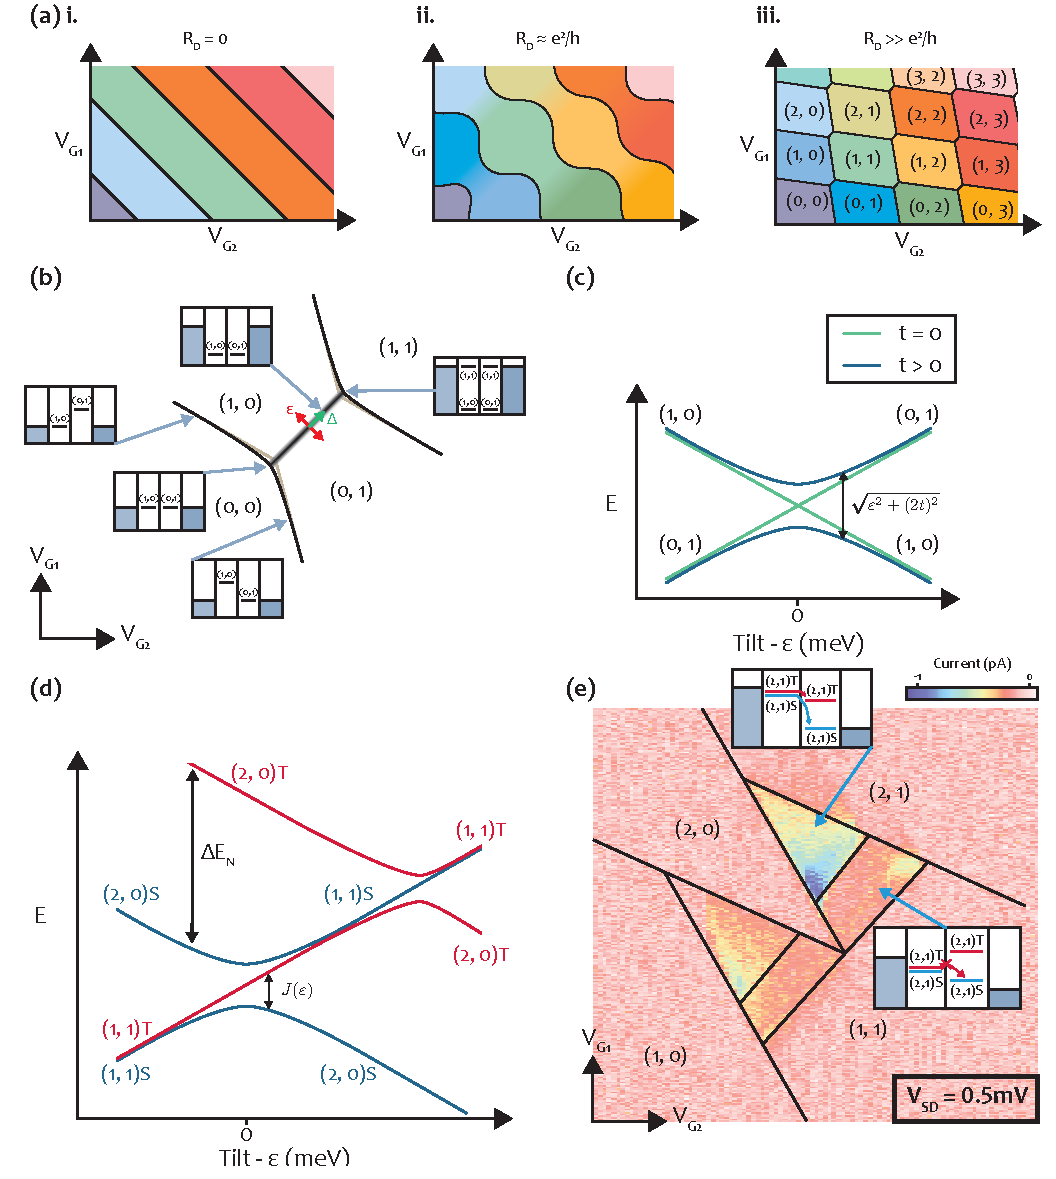
\includegraphics[width=0.9\linewidth]{ddenergy}
  \caption[Energy levels and spin in a double quantum dot]
  {\label{fig:dqdenergy}(a) Effect of varying $R_D$, the tunnelling rate between the two
  dots. At low resistance, the dot effectively reverts to a single quantum dot. As the resistance is increased towards
  $e^2/h$, two separated dots begin to form, although the transition between them is tunnel broadened.
  Finally, if the resistance is much larger than $e^2/h$, there are well defined transitions between left and right
  dot. (b) Zoom up of a single honeycomb cell around the $(0, 0)$, $(1, 0)$, $(0, 1)$ and $(1, 1)$ charge transitions.
  Insets show energy levels $\mu_1(N, M)$ of the left quantum dot and $\mu_2(N, M)$ of the right quantum dot where bracketed
  numbers indicate the charge occupancies of both dots. We define the tilt (offset) axes perpendicular (parallel) to the
  inter-dot transition in red (green). (c) Calculated energy levels along the $(0,1) \rightarrow (1,0)$ charge transition according
  to a full quantum model. For finite tunnel coupling, an avoided crossing is formed. (d) Calculated energies of singlet and
  triplet spin configurations for a two-electron double quantum dot. Due to the Pauli exclusion principle,
  the $(2, 0)T$ state is not accessible until we reach the first excited orbital state, such that the $(2, 0)T$ level is energetically
  inaccessible at zero tilt. We define the exchange energy $J(\varepsilon)$ as the energy between the $(1, 1)S$ and $(1, 1)T$
  states. (e) Current through a double quantum dot at $V_{SD} = \SI{0.5}{\milli\volt}$. Charge transitions split into finite bias triangles
  which reveal the presence of excited orbital states in the dot, as well as the effects of spin, which blocks transport through the orbital ground state of the dot.}
\end{figure}

The constant interaction model, however, has limited power to describe the effects of tunnelling between two dots,
as it assumes that the occupancy of each dot is a good quantum number, a situation which will not hold near
charge degeneracy points, specifically when tunnelling rates between the two dots is significant. If we wish to include a finite tunnel
rate, we must move to a Hubbard model that includes the effects of quantum fluctuations, spin and orbital states on each
dot \cite{PhysRevB.84.115301}. In this model, and indeed in most descriptions of double quantum dots, we
describe the strength of tunnelling between the two quantum dots as a \textbf{tunnel coupling}. This model allows us to draw a schematic
of the continuous evolution from a single quantum dot to a double quantum dot as the strength of the inter-dot tunnel coupling
is increased. For example, in Fig.~\ref{fig:dqdenergy} (a) we see the evolution from the case with large tunnel coupling (~zero tunnel resistance), i.e. a single
quantum dot in i., to a region of intermediate tunnel coupling in ii., and finally small tunnel coupling, i.e. a wholly separated quantum dot, in iii. In the
limit of smaller tunnel couplings (larger tunnel resistance), the bending of charge transitions will continue to be visible
at each charge transition as in Fig~\ref{fig:dqdenergy} (b), where the transitions of the constant interaction model (grey) are compared to
a full hubbard model (black).

We can examine in further detail a single honeycomb cell in the charge stability diagram of a dot that includes both a cross-capacitance and an inter-dot capacitance.
In the insets of Fig~\ref{fig:dqdenergy} (b) we map out the energy levels of a quantum dot at various points according to the constant interaction model.
In this case, looking at the $(0, 0), (0, 1), (1, 0), (1, 1)$ transition, we find two points where
three charge transitions meet, so-called triple points, where energy levels within both the left and right dot are aligned
with the reservoirs. If we were to try and pass a current through such a system, it would only be at these points that a
current would flow. In between these triple points we find a new inter-dot transition, which comes from the fact that $\mu_{(1 \textrm{~and~} 2)}$
is now a function of gate voltage \emph{and} the occupancy of dot $(2 \textrm{~and~} 1)$. This dependence on the
occupancy is a result of the inter-dot capacitance and leads to an additional penalty that must be
overcome to load an electron on both left and right dots. Hence, the point where we move to the $(1, 1)$ charge configration is
pushed up in both $V_{G1}$ and $V_{G2}$, and a $(0, 1) \rightarrow (1, 0)$ interdot transition appears. To further analyze this charge transition,
we rotate ourselves to align with the inter-dot transition and define two new perpendicular axes.
Tilt ($\varepsilon$) is defined as movement perpendicular to the interdot charge transition and is shown in red. It measures the relative
charge configuration of the dots ($\varepsilon = \mu_1 - \mu_2$) while keeping the overall charge of the two dots constant.
Offset ($\Delta$) is defined as movement parallel to the interdot charge transition and is shown in green.
It measures the total charge offset $\Delta = \mu_1 + \mu_2$ without modifying the relative distance between levels in the left
and right dot. In this way, we can move through the charge stability diagram in a way that ignores the effects of cross capacitances \cite{qubyte}.

Having defined the tilt axis, we can analyze in detail the inter-dot charge transition, which for moderate tunnel couplings will show
charge hybridization near the interdot charge transition. At these points, the charge becomes a bad quantum number and electrons become delocalized
across the two quantum dots, leading to a blurred charge transition [as sketched in Fig~\ref{fig:dqdenergy} (a) ii.]. If we calculate the energy
of the two charge states along the tilt axis, plotted in Fig.~\ref{fig:dqdenergy} (c), we find that a finite tunnel coupling leads to the
formation of an avoided crossing (blue), compared to no tunnel coupling (green), which at the centre will have a gap of $2t$. As a function of
tilt, we find the difference in the gap between the two states is:
\begin{equation}
  \Omega(\epsilon) = \sqrt{\varepsilon^2 + (2 t)^2}
\end{equation}
The charge hybridization also allows the measurement of tunnel coupling by measurement of the charge state near zero tilt,
which for intermediate tunnel couplings will vary smoothly between $(0, 1)$ and $(1, 0)$\cite{PhysRevLett.92.226801}.

\subsubsection{Spin}
The final effect we must include to describe the relevant physics is spin. Electrons are fermions, meaning
they have half-integer spin and obey the Pauli exclusion principle, an effect we've run into before when we considered
the filling of bands in a semiconductor. As a quick reminder, the spin of a system is described by the spin angular momentum operator
$S = [S_x, S_y, S_z]$ and a spin magnitude (principal spin) operator $S^2 \equiv S_x^2 + S_y^2 + S_z^2$. The three orthogonal projections of the spin
angular momentum are non-commuting, such that in general as long as we can choose a principal direction, we can describe the
state of a system with two quantum numbers: $S^2$ and $S_z$, where we have chosen $S_z$ by convention. The values of these operators
are:
\begin{eqnarray}
  S^2\ket{s, m_s} = \hbar^2s(s + 1)\ket{s, m_s} \\
  S_z\ket{s, m_s} = \hbar m_s\ket{s, m_s}
\end{eqnarray}
where you might see that the spin state is defined by two quantum numbers $s$, the \textbf{principle spin quantum number} that gives
us the total spin magnitude and $m_s$, the \textbf{azimuthal spin quantum number}, which gives us projections of the spin in different directions.
As with angular momentum, the value of $m_s$ varies in integer steps from $\{-s, -s+1, ..., s-1, s\}$. Therefore, for a single spin, we have two
eigenstates (again picking $S_z$ as our basis):
\begin{eqnarray}
  \ket{\uparrow} &= \ket{s = \tfrac{1}{2}, m_s = +\tfrac{1}{2}} \\
  \ket{\downarrow} &= \ket{s = \tfrac{1}{2}, m_s = -\tfrac{1}{2}}
\end{eqnarray}
At zero magnetic field in GaAs these two spin states are degenerate, however by application of a magnetic
field we are able to break the degeneracy of the states such that we can address the two spin states individually,
causing a spin splitting $\Delta E = g^* \mu_B B$ where $g^*$ is the Landé g-factor, $\mu_B$ is the Bohr
magnetron and $B$ is an externally applied magnetic field.

For systems with more than one spin, to find the states the system may occupy, we must take the
tensor product of the two individual spins:
\begin{equation}
  \ket{s_1, m_{s1}, s_2, m_{s2}} = \ket{s_1, m_{s1}} \otimes \ket{s_2, m_{s2}}
\end{equation}
Thus the spin states of the system are $\ket{\uparrow_1\uparrow_2}, \ket{\uparrow_1\downarrow_2}, \ket{\downarrow_1\uparrow_2}, \ket{\downarrow_1\downarrow_2}$
However, this representation gives us states in the basis of the two individual spins, which is less useful
when the two states are not easily separable, for example near a charge degeneracy point or when two electrons occupy a single dot.
It is often more useful to work in terms of total spin and azimuthal spin for the joint system, which we define in the following way:
\begin{eqnarray}
  S^2 &= (S_1 + S_2)^2 \\
  S_z &= S_{z1} + S_{z2}
\end{eqnarray}
Combining the spins, we find these four states are:
\begin{alignat}{2}
  \ket{S}   &= &\ket{s = 0, m_s = 0}   &= \frac{\ket{\uparrow\downarrow} + \ket{\downarrow\uparrow}}{\sqrt{2}} \\
  \ket{T_-} &= &\ket{s = 1, m_s = -1}  &= \ket{\downarrow\downarrow} \\
  \ket{T_0} &= &\ket{s = 1, m_s = 0}   &= \frac{\ket{\uparrow\downarrow} - \ket{\downarrow\uparrow}}{\sqrt{2}} \\
  \ket{T_+} &= &\ket{s = 1, m_s = +1}  &= \ket{\uparrow\uparrow}
\end{alignat}
In other words, we have a single state (the \textbf{singlet} state), where the two spins are opposite and hence
the total spin is zero ($s = 0$), and three states (the \textbf{triplet} states), where the two spins are equal ($s = 1$) and have
spin angular momenta that take the values $\{-1, 0, +1\}$. In the case that the two electrons occupy a single dot, the Pauli exclusion principle which tells
us that two equal spins cannot occupy the same orbital state (position) leads to the $(2, 0)T$ state having a higher
energy than the $(2, 0)S$ state with a gap set by the orbital states of the quantum dot $\Delta E_N$. This is
represented schematically in Fig.~\ref{fig:dqdenergy} (d), which shows the energy levels of a quantum dot around the
$(1, 1) \rightarrow (2, 0)$ charge transition as a function of tilt. Note that although the singlet state can freely
change state around zero tilt, a qubit in the triplet state will not transition into the $(2, 0)$ charge configuration
until we can populate an excited orbital mode off to the right. This effect is visible in the current through a double
quantum dot, which will undergo a rectification due to this spin blockade, as shown in Fig~\ref{fig:dqdenergy} (e).
Here, we find two finite bias triangles, which are the double quantum dot equivalent of Coulomb diamonds \cite{PhysRevB.72.165308}.
Charge transport through the quantum dots proceeds via a sequence of electron tunneling events. In the forward direction
these would be: $(2, 1) \rightarrow (2, 0) \rightarrow (1, 1) \rightarrow (2, 1)$, a sequence that transfers a single electron
from the left to the right reservoir. Note that near zero tilt, only a singlet state may be loaded into the left dot
in the $(1, 1) \rightarrow (2, 1)$ transition; however, since we have an effectively infinite source of electrons in the
reservoir, this can be easily accomplished. In the reverse direction, the situation depicted in the figure, electrons flow
from the right to the left reservoir via the path $(2, 1) \rightarrow (1, 1) \rightarrow (2, 0) \rightarrow (2, 1)$.
In this direction, the charge transition $(1, 1) \rightarrow (2, 0)$ will be blocked depending on the spin of the right
electron, until the second orbital energy level is accessible, a situation depicted in the insets of Fig.~\ref{fig:dqdenergy} (e).
The prevented transition leads to a region of blocked current near the base of the triangle and a reemergence of current once the second orbital
becomes accessible or spin relaxation occurs.

As with single spins, away from any charge degeneracy points, these four states are all degenerate. Near zero tilt we get an
energy difference that opens between the singlet and triplet states called the exchange energy $J(\varepsilon)$. At this
point, the triplet state is doubly degenerate between the $T_-$, $T_0$ and $T_+$ states. Application of a magnetic field creates
a splitting between these three levels given by $\Delta E = g^* \mu_B B S_z$, which causes no change to the $S$ and $T_0$ state,
and causes the $T_+$ and $T_-$ states to split off around the $T_0$ state. This will useful for defining our two-level subsystem
in our discussion of singlet-triplet qubits later on.

\subsubsection{Defining Double Quantum Dots on GaAs}

\begin{table}
  \centering
  \begin{tabular}{|l|c|l|}
   \hline
   Lattice Constant (\si{\angstrom}) & $a$ & 5.65 \\ \hline
   Dielectric Constant & $\epsilon_r = \tfrac{\epsilon}{\epsilon_0}$ & 12.9 \\ \hline
   Land\'e g-factor & $g^*$ & -0.44 \\ \hline
   Electron Effective Mass & $(m^*/m_e) $ & 0.066 \\ \hline
   2DEG Depth (\si{\nano\meter}) & $d$ & 91 \\ \hline
   Density (\si{\per\square\centi\meter}) & $n_s$ & $1.30 \times 10^{11}$ \\ \hline
   Mobility (\si{\square\centi\meter\per\volt\per\second}) & $\mu$ & $4.8 \times 10^6$ \\ \hline
   Fermi Wavelength (\si{\nano\meter}) & $\lambda_F = \sqrt{\frac{2 \pi}{n_s}}$ & 70 \\
   \hline
  \end{tabular}
  \caption[Representative properties of a GaAs 2DEG used for forming quantum dots]
  {Representative properties of a GaAs 2DEG used for forming quantum dots, based on material
  grown by the group of Mike Manfra at Purdue University.}
  \label{tab:gaas2deg}
\end{table}

Having covered the theoretical description of a quantum dot as well as the physics behind the 2DEG, we can
describe the formation of a quantum dot in GaAs. Typical parameters for a 2DEG in GaAs are given in able~\ref{tab:gaas2deg}, however,
the key properties we require are the Fermi wavelength, which will set the approximate size of the dot we wish
to form, and the depth, which will set the sharpness of the potential that the gates provide at the 2DEG. For samples that are
doped and have an intrinsic density of electrons, we can form quantum dots by evaporating surface gates on top of an insulating
dielectric [usually TiAu on top of $\approx \SI{10}{\nano\meter}$ \ce{HfO2} or \ce{Al2O3}, as shown in Fig.~\ref{fig:heterostructure} (c)],
and applying negative voltages to deplete electrons below the gate in the 2DEG. Initially, we expect the gate to change
the density at the 2DEG as per that of a parallel plate capacitor:
\begin{equation}
  \Delta n_s = \frac{\epsilon_r \epsilon_0 \Delta V_g}{e d}
\end{equation}
For a gate at depth $d = \SI{101}{\nano\meter}$ from a 2DEG with density $n_s = \den{1.3e11}$ we expect depletion at around $V_g = \SI{-180}{\mv}$.
After this, increasingly negative gate voltages deplete the 2DEG in a halo around the gate.

Contact is made to the 2DEG via metallic ohmic contacts formed using a eutectic alloy of AuGe, which after evaporation is annealed
at approximately \SI{450}{\celsius}. A full description of the fabrication process which gives ratios and thicknesses is given
in Appendix~\ref{sec:fab}, for now, all we need to know is this n-dopes the semiconductor directly under the contact with Germanium
causing a contact to be formed to the 2DEG with a resistance of between \SI{20}{\ohm} and a few \si{\kilo\ohm} depending on the size and quality
of the ohmic contact.

\begin{figure}
  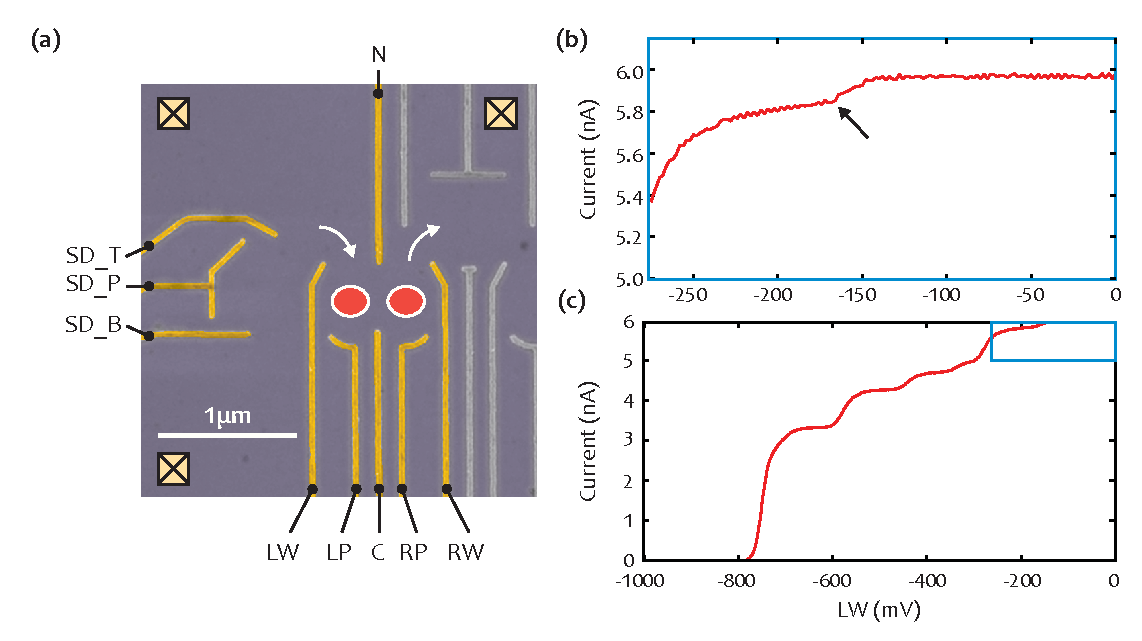
\includegraphics[width=0.9\linewidth]{Device}
  \caption[SEM image of a double quantum dot on GaAs]
  {\label{fig:dd_design}(a) False color SEM of a double quantum dot design on GaAs. Surface gates (highlighted in gold) are
  12nm TiAu onto which negative voltages are applied to deplete the 2DEG 101nm underneath. The locations of the quantum dots are
  highlighted with red circles and the ohmic contacts to the 2DEG in yellow boxes. Descriptions of the gates are given in the
  main text. The width of the double quantum dot at the surface is 970nm. (b) The left wall passing through depletion while
  pinching off with the nose (set to -800mV), at the location marked with the arrow. All other gates are at zero. (c)
  A full pinch-off curve of the left wall against the nose. As the undepleted region of the 2DEG shrinks towards the Fermi
  wavelength, a 1D channel is formed, causing the appearance of quantized conductance plateaus.}
\end{figure}

The design of gate structures that can confine electrons into quantum dots is an area of continued and fruitful research (see for
example Section~\ref{sec:5dot} of this thesis), however a common and well-tested pattern for a double quantum dot is shown in Fig.~\ref{fig:dd_design} (a).
Gates are designed to correspond to the various parameters we described in Section~\ref{sec:qd}; with the gates labelled LW (left wall)
and RW (right wall) controlling the tunnel rates from the reservoirs to the dots, the gate labelled C (centre) controlling the tunnel coupling
$t_c$, and LP (left plunger) and RP (right plunger) controlling the chemical potential of the left dot ($\mu_1$) and right dot ($\mu_2$) respectively.
The N (nose) gate acts as a global control, and a charge sensor (discussed in Section~\ref{sec:readout}) which in this case is a third quantum dot formed
against the left wall is placed to the left of the device. The location of ohmic contacts is marked by crosses and allows us to measure current both
through the device and through the sensor.

The left wall of the quantum dot passing through depletion is shown in Fig.~\ref{fig:dd_design} (b) at the
location marked by the arrow. A full pinch-off trace for the gate is given in Fig.~\ref{fig:dd_design} (c), showing the appearance of quantized
conductance steps as the undepleted region of 2DEG shrinks to towards the Fermi wavelength. These steps appear in units of the spin-degenerate conductance quantum,
$R = 2 n e^2/h$ for integer $n$, the physics of which we discuss in more detail in Section~\ref{sec:char}. Several gates on the device
are wired up to allow the application of radio frequency tones or fast pulses to drive qubit rotations.
Further details of how this is accomplished are given in~\ref{sec:setup}.

\subsection{Qubits from Quantum Dots}
\label{sec:dotqubits}
As we discussed at the beginning of this section, one of the challenges of quantum computing is finding physical systems
suitable to be used as qubits. They must be expressible as a two-level system, isolated enough that the quantum state is
preserved during operations, and easily read-out and controlled. The last of these requirements is effectively the
same as finding a system whose Hamiltonian ($H$) can express the operations that we defined in Section~\ref{sec:qc}. We use
Schrödinger's equation to describe this evolution:
\begin{equation}
  i \hbar \diff{\ket{\psi(t)}}{t} = H \ket{\psi(t)}
\end{equation}
For this reason, Hamiltonians describing two level systems used in quantum computers are often explicitly defined in terms of
the Pauli matrices we defined in equation~\ref{eq:pauli}. For example, a model qubit Hamiltonian may be given by:
\begin{equation}
  H = A \sigma_X + B \sigma_Z = \svec{B&A\\A&-B}
\end{equation}
which describes rotations around an axis of the Bloch sphere at angle $\theta = \tan^{-1}\left(\tfrac{A}{B}\right)$ and with a rate
$\omega_r = \tfrac{\sqrt{A^2 + B^2}}{\hbar}$. By varying the values of $A$ and $B$, we are able to construct arbitrary
rotations around the Bloch sphere. Alternatively, the application of photons at the frequency
$\omega_e = 2\sqrt{A^2 + B^2}$ is able to drive transitions between the eigenstates of this Hamiltonian.

\subsubsection{The Charge Qubit}
Perhaps the simplest form of qubit we can form with a double quantum dot system is a charge qubit. Here we define
the logical subspace of the qubit as spanned by two charge states, typically the $(0, 1)$ and $(1, 0)$ charge states,
with the basis $\ket{0} = (0, 1)$ and $\ket{1} = (1, 0)$. The single qubit Hamiltonian is given by:
\begin{equation}
  H_{\textrm{charge}} = \frac{1}{2}\varepsilon\sigma_Z + t_c\sigma_X
\end{equation}
which is represented by the energy level diagram in Fig.~\ref{fig:dqdenergy}. The qubit is typically operated by the application
of microwave pulses with frequency $\Omega = \sqrt{\varepsilon^2 + (2 t_c)^2}$ in order to drive transitions between the ground and
excited charge configurations, and the state is read out via a proximal charge sensor (discussed in Section~\ref{sec:readout}).

Such a qubit, while conceptually simple is highly sensitive to charge noise in the semiconductor, such that the qubit lifetime $T_1$ and
coherence times $T_2$ are both on the order of \SI{10}{\nano\second}\cite{PhysRevLett.105.246804}. As such, the usefulness of such a qubit
is limited.

\subsubsection{The Loss-DiVincenzo (Single Spin) Qubit}
The next idea for the implementation of a qubit would be to use the spin of a single electron as our two-level subsystem. In
many ways, spin is an ideal phenomenon to use. It is naturally two levels, and as such has no leakage states that our qubit
may accidentally end up in and can easily be implemented using quantum dots \cite{PhysRevA.57.120}. We can represent the $\ket{0}$ and $\ket{1}$ states
by the spin down and up states ($\ket{\downarrow}$ and $\ket{\uparrow}$) respectively. The splitting between the two states
is controlled by the application of an external magnetic field that causes a Zeeman splitting $\Delta E_Z = g^* \mu_B B$. Since the
spin of an electron does not couple to electric fields (to first order), this gives the single-spin qubit some resistance to
charge noise in the semiconductor. Of course, this also makes the control of the qubit more challenging, as we now require
an oscillating magnetic field to control the qubit. As such, the Hamiltonian, and the control of such a qubit will vary depending on
how we achieve our qubit control. There are four common methods described in the literature for controlling
single spin qubits:
\begin{enumerate}
  \item \textbf{Electron Spin Resonance (ESR)} An alternating magnetic field is generated by an alternating current run through a proximal ESR gate,
        with a frequency matching the Zeeman splitting \cite{nnano.2014.216}. However, this method of driving rotations is relatively
        slow (on the order of a few \si{\micro\second}) and requires large microwave powers.
  \item \textbf{Electron-Dipole Induced Spin Resonance (EDSR)} In materials with strong spin-orbit interaction, we can
        use the effective magnetic field felt by an electron in motion in a confining potential. Such techniques utilize an AC electric
        field to "wobble" the electron wave function to drive rotations within a single dot \cite{Nowack1430,nature11559}. This technique
        achieves spin rotations in $\approx \SI{100}{\nano\second}$ in GaAs, down to $\approx \SI{10}{\nano\second}$ in InAs with a stronger spin-orbit coupling.
  \item \textbf{Electrically-Driven ESR in a Slanted Magnetic Field} In materials without strong spin-orbit interaction,
        we can generate an effective oscillating magnetic field by generating a strong magnetic field gradient across a quantum dot with the use of a micromagnet.
        Again, the "wobble" of the electron wave function drives rotations of single spins in a single dot \cite{PhysRevLett.107.146801}
        or between two quantum dots \cite{2019arXiv190500346C}. This technique allows rotations on the order of $\approx \SI{10}{\nano\second}$.
  \item \textbf{Electrically-Driven ESR in the Exchange Field of an Auxilliary Spin} The use of an auxiliary spin against
        which we can drive rotations via the exchange interaction again  allows electric field control of spin with sub-nanosecond operation times \cite{PhysRevB.90.235311}.
        In many ways, this method of control is similar to that of the singlet-triplet qubit, described below, with the exception that we still use a single
        spin as our logical subspace. However, such control has not yet been realized.
\end{enumerate}

As mentioned above, although we have first-order insensitivity to electric fields, the slow speed of ESR leads us to
reintroduce an electric field coupling, either via intrinsic material properties via the spin-orbit interaction, or through
the creation of gradient magnetic fields, to allow for fast control of these qubits. Even then the effect of charge noise
is far lower than for a charge qubit, with coherence times of hundreds of microseconds possible. Additional sources
of noise originate from the coupling between electron spins and the nuclear spins of nearby spinful nuclei. This
effect is termed the Hyperfine interaction, and leads to a fluctuating field, termed the Overhauser field, with magnitude:
\begin{equation}
  B_{\textrm{nuc}} = \frac{1}{g^* \mu_B} \sum^N_n A_nI_n
\end{equation}
where $I_n$ is the nuclear spin operator for the n-th nucleus, and $A_k$ is the coupling strength of that nucleus with the
electron spin. We can treat the Overhauser field as a classical random variable with a Gaussian distribution around zero net
polarization. The RMS fluctuation of $B_{\textrm{nuc}}$ is $\sigma_B = \tfrac{\SI{4.0}{\tesla}}{\sqrt{N}}$ where N is the number of
nuclei that an electron in a quantum dot overlaps \cite{PhysRevB.76.035315}. For GaAs this is typically on the order of $N \approx 10^6$.
This effect is minimized by the use of isotopically purified silicon \cite{itoh_watanabe_2014}, which contains a
reduced density of spinful nuclei.

\subsubsection{The Singlet-Triplet Qubit}
The use of a single spin, while having a convenient mapping to qubit states, requires either the application of an AC magnetic field
or an AC electric field coupled with some form of gradient magnetic field or spin-orbit interaction. By creating ensembles of
spin, we can trade off a more straightforward system for one with more flexible control or greater immunity to certain types of noise.
The use of two electrons across two quantum dots allows us to use purely pulsed DC control to achieve full control
over the qubit. For this type of qubit, we define our computational subspace as spin states of two coupled electrons, choosing
$\ket{S}$ and $\ket{T_0}$ as our $\ket{0}$ and $\ket{1}$ state respectively, with a Hamiltonian described by:
\begin{equation}
  H = J(\varepsilon)\sigma_Z + g^* \mu_B \Delta B_X \sigma_X
\end{equation}
The fixed gradient field $\Delta B_X$ is achieved either through the use of a micromagnet or via the polarization of the nuclear
field \cite{PhysRevLett.105.216803}, where $\Delta B_X$ describes the difference in the field seen by an electron in the left and
right quantum dots. An external magnetic field is required to break the degeneracy of the three triplet states, such that
we only operate in the $S-T_0$ states. Any leakage into the $T_-$ or $T_+$ states is undesirable.

\begin{figure}
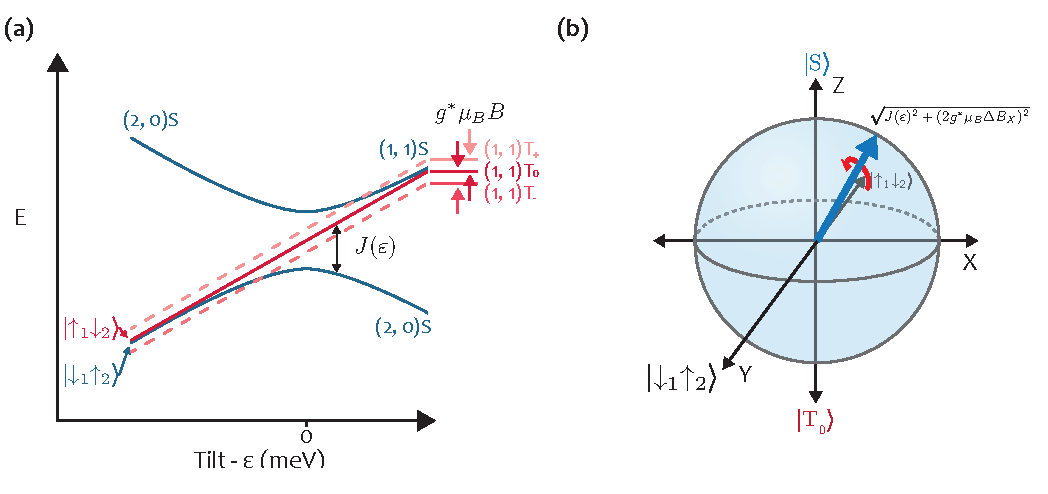
\includegraphics[width=0.95\linewidth]{st0}
\caption[Energy levels and eigenstates of a Singlet-Triplet qubit]
{\label{fig:st0}(a) The energy levels of a Singlet-Triplet Qubit. The three triplet states are split by the application of a
uniform magnetic field $B$. At a large negative tilt, i.e. $J(\epsilon) \approx 0$, the gradient magnetic field $\Delta B_X$ leads to a
change in basis, such that the energy eigenstates are described by $\ket{\uparrow_1\downarrow_2}$ and $\ket{\downarrow_1\uparrow_2}$,
where here we've arbitrarily chosen $\Delta B_X > 0$.
(b) Bloch sphere representation of a single Singlet-Triplet qubit. Qubit rotation proceeds around the axis in blue,
which may be varied by pulsing tilt ($\varepsilon$). The gradient field $\Delta B_X$ is usually constant, set either
by nuclear fields or a fixed micromagnet.}
\end{figure}

The energy levels of such a qubit are shown in Fig.~\ref{fig:st0} (a). The qubit may be easily initialized in the $(2, 0)S$ state via
the exchange of electrons with the reservoirs, as the $(2, 0)T$ states are energetically inaccessible for small tilt and offset [as we
saw in~\ref{fig:dqdenergy} (d)]. In general, $S-T_0$ qubit rotations are driven around an axis set by the relative magnitudes
of $J$ and $\Delta B_X$, as is shown in Fig.~\ref{fig:st0} (b), however, by pulsing tilt, we are able to drive rotations around the Z axis
when $J(\varepsilon) \gg g^* \mu_B \Delta B_X$, or around the X-axis when $g^* \mu_B \Delta B_X \gg J(\varepsilon)$. An equivalent way of
expressing this is to speak in terms of energy eigenstates: for large $J(\varepsilon)$, the two eigenstates of the qubit are $\ket{S}$ and
$\ket{T_0}$, while for $J(\varepsilon) \approx 0$, the energy eigenstates of the qubit are set by the gradient field $\Delta B_X$, with
the ground state given by spins anti-aligned with the gradient magnetic field (since $g^* < 0$ in GaAs), and the excited state by spins aligned with
the gradient magnetic field. Lifetimes for singlet-triplet qubits are primarily limited by coupling to nuclear spins via the hyperfine
interaction \cite{nnano.2016.170}, which causes fluctuations in the coefficient of $\sigma_X$, as well as charge noise that is ever present
in semiconductor-based systems \cite{PhysRevLett.110.146804}. Despite this, coherence times have been extended in GaAs spin qubits to
over \SI{200}{\micro\second} via the use of dynamical decoupling sequences \cite{nphys1856}.

It is also worth mentioning that there is active research in optimizing the control schemes for singlet-triplet qubits, again with
the intention of gaining resistance to certain forms of noise. For example, recent results suggest that variation of $J(\varepsilon)$ by modulation of
tunnel coupling $t_C$, leading to symmetric pulses on the left and right quantum dot \cite{PhysRevB.73.205302,PhysRevB.97.155402,PhysRevLett.116.116801,PhysRevLett.118.216802},
or the use of magnetic field gradient estimation and active control \cite{ncomms6156,s41534-016-0003-1} may lead to higher
fidelity control and reduced dephasing. Further reduction in charge noise is expected with
improved materials growth, which is expected to further extend qubit coherence times \cite{PhysRevApplied.9.034008}.

\subsubsection{The Exchange-Only Qubit}

\begin{figure}
  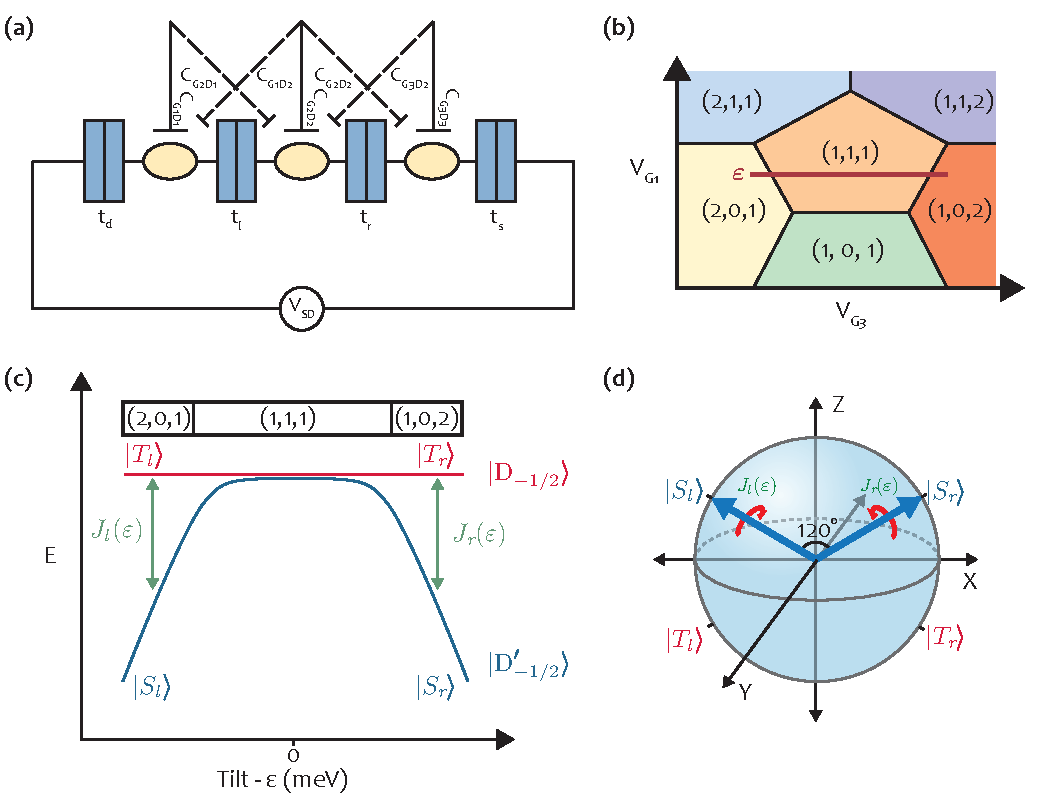
\includegraphics[width=0.95\linewidth]{eo}
  \caption[Energy levels and eigenstates of an Exchange-Only qubit]
  {\label{fig:eo}(a) Schematic of a triple quantum dot, with tunable tunnel couplings between the left and centre quantum dots, and the
  right and centre quantum dots. (b) Charge stability diagram for a triple quantum dot when sweeping the $V_{G1}$ and $V_{G3}$ around the
  $(1,1,1)$ charge configuration. The tilt axis is marked in red and sweeps from the $(2,0,1) \rightarrow (1,1,1) \rightarrow (1,0,2)$
  charge configurations. (c) Energy levels of the exchange-only qubit. Quadruplet states or excited doublet states are not shown. The Exchange energies
  between the left (right) and centre dots are swept as a function of tilt. The energy eigenstates change between $\ket{S/T_l}$ and $ket{S/T_r}$
  at the extremes of tilt. (d) Bloch state representation of the exchange-only qubit. The exchange interaction drives rotation around two
  axes of the Bloch sphere separated by \SI{120}{\degree}.}
\end{figure}

While the singlet-triplet qubit described in the above section allows us to control our qubits with only fast pulses, they still require
a spatially varying magnetic field for full two-axis control. The use of three electrons distributed through three quantum dots allows
for fully electrical control of a spin qubit using only exchange interactions between the left and centre, and right and centre quantum
dots \cite{10.1038-35042541}, as shown in Fig~\ref{fig:eo} (a) and (b). In this case, the system has a total of eight possible spin states. These
are one set of quadruplet states with total spin $S^2 = 3/2$ and spin projections $S_Z = \{-3/2, -1/2, +1/2, +3/2\}$, and two sets of doublet
states corresponding to a singlet or triplet in the left (right) dot, and a third spin on the right (left) dot. The choice of placing the singlet/triplet
state on the left or right dot is set by the tilt, with the energy eigenstates of the system given by the singlet/triplet state on the left for $\varepsilon \ll 0$,
and on the right for $\varepsilon \gg 0$. We can, therefore, write out the four doublet states as
\footnote{The full set of eigenstates at different values of $J_l, J_r, \varepsilon$ can be found in \cite{PhysRevB.82.075403}}:
\begin{equation}
\begin{split}
  \ket{\textrm{D}_{-1/2}}        &= \ket{\uparrow T_R}   (\textrm{for }\varepsilon \gg 0) = \ket{T_L\uparrow}   (\textrm{for }\varepsilon \ll 0)\\
  \ket{\textrm{D}_{+1/2}}        &= \ket{\downarrow T_R} (\textrm{for }\varepsilon \gg 0) = \ket{T_L\downarrow} (\textrm{for }\varepsilon \ll 0)\\
  \ket{\textrm{D}^\prime_{-1/2}} &= \ket{\uparrow S_R}   (\textrm{for }\varepsilon \gg 0) = \ket{S_L\uparrow}   (\textrm{for }\varepsilon \ll 0)\\
  \ket{\textrm{D}^\prime_{+1/2}} &= \ket{\downarrow S_R} (\textrm{for }\varepsilon \gg 0) = \ket{S_L\downarrow} (\textrm{for }\varepsilon \ll 0)\\
\end{split}
\end{equation}

In order to break the degeneracy of the third spin, a global magnetic field is applied, such that we are left with our computational basis states, which
I arbitrarily choose to be the $-1/2$ states here:
\begin{alignat}{2}
  \ket{0} &=& \ket{\textrm{D}^\prime_{-1/2}} &= \ket{S_{l,r}} \\
  \ket{1} &=& \ket{\textrm{D}_{-1/2}} &= \ket{T_{l,r}}
\end{alignat}

Focussing on this subspace, the energy level diagram of the exchange-only qubit is given in Fig.~\ref{fig:eo} (c). We are able to change the exchange
energy between the left (right) and center dots by sweeping tilt ($\varepsilon$). We can largely ignore leakage states as the set of four quadruplet
states have different principal spin, and the two remaining doublet states are rendered inaccessible by the applied Zeeman field. The exchange-only
qubit was first experimentally realized in \cite{PhysRevB.82.075403}. In GaAs systems, rotations at rates of up to \SI{47.4}{\giga\hertz} have been measured,
with a lower bound of $T_2 = \SI{100}{\nano\second}$, limited by nuclear spins in GaAs \cite{nnano.2013.168}.

The fast rotation rate also leads to increased sensitivity to exchange (charge) noise, however improved schemes building
on the ideas of the exchange-only qubit \cite{Russ_2017}, such as the Resonant Exchange Qubit \cite{PhysRevLett.111.050501},
the Always-On Exchange-Only (AEON) qubit \cite{PhysRevB.93.121410} or the Quadrupolar Exchange-Only Qubit \cite{PhysRevLett.121.177701,Kornich_2018},
which trade off the number of electrons or requirements to continuously drive the system for insensitivity to certain forms of noise.
Additional work with double quantum dots with higher electron occupancies and hence higher principal spin quantum numbers are also
predicted to have desirable noise rejection, while still allowing fully electrical control, such as the hybrid
spin/charge-qubit \cite{PhysRevLett.108.140503}, which has recently shown an ensemble dephasing time
of $T_2^* = \SI{8.1}{\nano\second}$ with rotation rate $f_{\textrm{rabi}} = \SI{2.43}{\giga\hertz}$ in
GaAs \cite{PhysRevLett.116.086801} or $T_2^* = \SI{2}{\nano\second}$ with rotation rate $f_{\textrm{rabi}} = \SI{5.2}{\giga\hertz}$ in
Si/SiGe \cite{nature13407}, which is presently limited by charge noise \cite{s41534-017-0034-2}.

\subsection{Majorana Zero Modes}
\label{sec:majo}

While the above section runs through several techniques for building qubits using semiconductor heterostructures,
each of them suffers from a significant amount of noise that must be corrected for these qubits to be useful
in a quantum computer. For an error rate of $1 \times 10^{-5}$, it is estimated that roughly 3,000 physical qubits
are required to construct one logical qubit using the surface code, and close to 10,000 gates must be performed per computational gate, to correct
errors as the occur \cite{6657074}. For spin qubits, although single qubit gate fidelities routinely exceed $99\%$\cite{Zajac439}, two-qubit
gate fidelities of 98\% are the highest values the author is aware of at the time of writing \cite{PhysRevA.99.042310}.
The source of error, as we discussed in previous sections, is caused by uncontrolled coupling to the environment, causing the information stored in the qubits
to be lost. An alternative approach to building qubits, one that uses the topology of exotic quasiparticles called non-abelian anyons,
was proposed by Kitaev as a method of performing quantum computation in a way that is protected from local peturbations \cite{KITAEV20032}.

A system of non-abelian anyons uses as it's computational subspace a set of degenerate ground states with a fixed number
of quasiparticles, separated by a physical distance, where information is stored over multiple pairs of anyons. A result of this
distributed storage is that any local perturbation to a quasiparticle does not
lead to decoherence. To quote: \textquote[{\cite{RevModPhys.80.1083}}]{the only way the system can undergo a non-trivial unitary evolution ---
that is an evolution that takes it from one ground state to another --- is by having its quasiparticles braided}. A physical movement or
interaction of pairs of anyons is required to change the state of the qubit. In such a way, error rates
far below those achievable in other qubit systems may be possible. Rather than requiring many noisy qubits to form one logical qubit,
we would be able to use a few, or even a single clean qubit instead. I will not go into further details of how such a computation
is achieved via braiding, but will point the interested reader towards \cite{RevModPhys.80.1083}, which
gives a far more thorough introduction to the physics than I can in the limited space I have available. I will, however, give a quick introduction
into the physical origins of the Majorana zero mode, based on the material from \cite{rafael_notes}.

\begin{figure}
  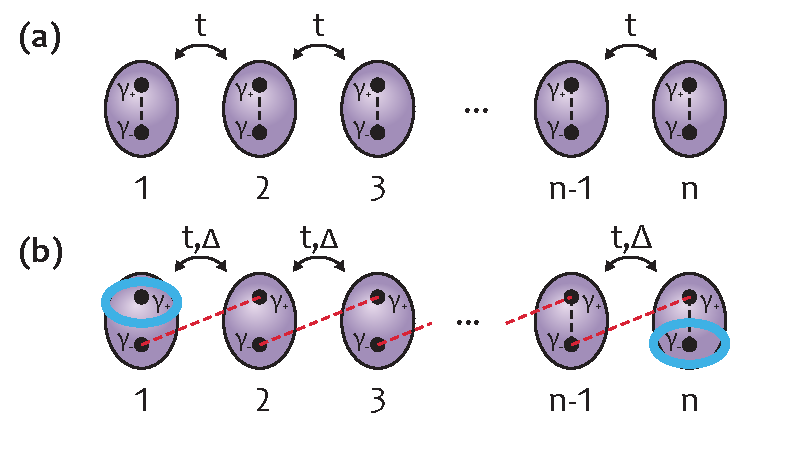
\includegraphics[width=0.65\linewidth]{majochain}
  \caption[1D chain of fermions, forming a Majorana zero modes]
  {\label{fig:majo}(a) Schematic of a 1D chain of fermions under conventional pairing. Although each fermion is broken into two
  Majorana operators, each pair of operators are tied to a single real particle, and we cannot manipulate them in isolation.
  (b) A chain where $\mu = 0$ and $\Delta = t \neq 0$. In this configuration the pairing occurs between neighbouring Majorana operators,
  leaving two unpaired Majorana zero modes (blue) at either end of our chain. We can use four of these unbound states as a
  topologically protected qubit.}
\end{figure}

The challenge, then, is to find a system which contains these emergent quasiparticles. Again, it was Kitaev that proposed that
a one-dimensional chain of fermions, with a specific Hamiltonian, may cause the emergence of precisely the quasiparticles we require \cite{Kitaev_2001}.
The Hamiltonian he proposed was \cite{Alicea_2012}:
\begin{equation}
  H = -\mu\sum_j \hat c_j^\dagger \hat c_j - \frac{t}{2}\sum_j\left(\hat c_j^\dagger \hat c_{j+1} + \hat c_{j+1}^\dagger \hat c_j\right)
      -\frac{\Delta}{2}\sum_j\left(e^{i\phi}\hat c_j\hat c_{j+1} + e^{-i\phi} \hat c_{j+1}^\dagger \hat c_j^\dagger\right)
  \label{eq:kith}
\end{equation}
Here we have a set of sites, indexed by $j$, with an onsite energy (chemical potentital) $\mu$, a hopping term $t$, and a superconducting coupling
term $\Delta$ with phase $\phi$. The terms $\hat c_i$ and $\hat c_i^\dagger$ are the fermion annihilation and creation operators respectively.
Let's look at a few limits of this Hamiltonian. For $\mu < 0$ and $\Delta, t = 0$, this Hamiltonian describes a wire with a single ground state containing a fixed
number of fermions. If we wish to add an extra electron, we must pay an energy cost $\mu$, as in Fig.~\ref{fig:majo} (a). The next case we consider is where $\mu=0$ and
$\Delta = t \neq 0$. We can achieve the first requirement by coupling the wire strongly to a large reservoir of fermions, such that the number of
fermions on the wire is not a good quantum number (exactly the opposite of a quantum dot). To understand the effect of the next two terms, it is
helpful to decompose the fermion annihilation and creation operators into Majorana operators:
\begin{align}
  \gamma_+ = \hat c + \hat c^\dagger && \gamma_- = -i(\hat c - \hat c^\dagger)
\end{align}
These are real operators ($\gamma_\pm = \gamma_\pm^\dagger$), they square to 1 ($\gamma_\pm^2 = 1$), and they anticommute ($\left\{\gamma_+, \gamma_-\right\} = 0$).
Indeed there is nothing special about these operators; I could easily define them for a single fermion state, which would yield:
\begin{align}
  \hat c = \frac{1}{2}(\gamma_{+} + i\gamma_{-}) && \hat c^\dagger = \frac{1}{2}(\gamma_{+} - \gamma{-})
\end{align}
however since both operators are associated with a single wave function, they are inseparable. In fact, I have even drawn my fermions in Fig.~\ref{fig:majo} (a) as a
pair of Majorana operators. There is really only one state described by the two operators.
The question we need to answer is how do we separate our Majoranas. Let's write down the Kitaev Hamiltonian from Equation~\ref{eq:kith}
substituting in our Majorana operators. After some rearrangement (and the removal of a global phase) we find:
\begin{equation}
  H = -\frac{\mu}{2}\sum_j(1 + i\gamma_{j,+}\gamma_{j,-}) - \frac{t + \Delta}{4}\sum_j i \gamma_{j,-}\gamma_{j+1,-} - \frac{\Delta - t}{4}\sum_j i \gamma_{j,+}\gamma_{j+1,-}
\end{equation}
Note a number of features: $P_i = (1 + i\gamma_{j,+}\gamma_{j,-})$ gives us the parity of the site $i$, and the second and third terms give inter-site Majorana couplings.
For $\mu < 0$ and $\Delta, t = 0$ we recover the original description of a wire with a set of occupied or unoccupied sites. In the case
that $\mu = 0$ and $\Delta = t \neq 0$, we end up with a vacuum state, gapped from the next state by $\tfrac{\Delta+t}{4}$, but with two unpaired
Majorana zero modes $\gamma_{0,+}$ and $\gamma_{N,-}$, which form a zero-energy two-level system. They are protected from local perturbations
by their non-local nature, a situation depicted in Fig.~\ref{fig:majo}. In fact this "topological" domain extends around the region of $\Delta = t \neq 0$
allowing us to construct fault-tolerant qubits out of 2 pairs of Majorana zero modes \cite{RevModPhys.80.1083}.

The experimental challenge is to find a physical system that is similar to that described by the Hamiltonian in Equation~\ref{eq:kith}. We can make a 1D chain using the principles
we've covered up to this point, and the electron pairing is similar to that of a superconductor, the complication is that the Hamiltonian describes
a set of spinless fermions. The spin of electrons would, unfortunately, prevent the pairing described above. We will cover one such method for forming
a spinless 1D superconductor in Sec.~\ref{sec:makemajo}, which combines a superconducting 1D system with strong spin-orbit coupling and a
parallel magnetic field to create an effective spinless system \cite{PhysRevLett.105.077001,PhysRevLett.105.177002}. At this point, such systems
have been experimentally realized, and evidence for the existence of Majorana zero modes is mounting \cite{Mourik1003,s41578-018-0003-1}, however as of writing
a topologically protected qubit has not yet been observed.

\section{Characterizing 2DEGs}
\label{sec:char}
In the previous sections, we went through how a 2DEG is constructed and wrote down some equations for scattering
and conductivity in a 2DEG. These equations have all assumed that the 2DEG is purely classical, however at the temperatures
and scales that many of our devices operate, this assumption begins to break down. To explore why this is the case,
we must revisit the scattering mechanisms and equations for conductance that we previously wrote down in Equation~\ref{eq:cond}
and add some quantum corrections to these equations. As we do this, we can define several regimes for transport
where various quantum corrections to transport become apparent.

Before we get started, let's quickly review the scattering lengths that we originally defined in Section~\ref{sec:2deg}. We can classify
scattering into two forms, elastic scattering, which occurs when the electron changes direction but not its energy or wavevector, or
inelastic scattering, which occurs when the scattering event changes the energy of the electron. Elastic scattering occurs at impurities, or along dislocations
and walls, i.e. on scattering sites with a mass much larger than the electron itself. The distance between successive elastic scattering events is
called the elastic scattering length $l_e$\footnote{This is sometimes also called the momentum relaxation length, $l_m$ or $l_{\textrm{imp}}$.}.
Inelastic scattering occurs via time-dependent mechanisms such as phonons or electron-electron scattering. As the scatterers have energy and
mass on the order of the electron energy and mass, the electron and the scatterer transfer energy readily. In 2DEGs, our assumption that
electrons do not interact continues to hold for the effects we wish to explore, and hence, the primary inelastic scattering mechanism is electron-phonon scattering.
As phonons are largely thermally generated, inelastic scattering, therefore, occurs on the length-scale $l_i$, set by the temperature of the sample. Since these scattering events
are each unique and time-dependent, the events effectively randomize the phase of the electron, and so
the inelastic scattering length $l_i$ is often used interchangeably with $l_\phi$, the phase coherence length.

We now have the ingredients necessary to classify transport into several distinct regimes, based on the relationship between the size
of the system being measured $L$, and the various length scales in our system $l_\phi$, $l_e$ and $\lambda_F$.
\begin{itemize}
  \item \textbf{Classical Diffusive} ($\lambda_F < l_e, l_\phi \ll L$): This is the classical limit of transport, true for large pieces of metal or semiconductor. The system is much larger than any relevant scattering length; hence, electrons travel diffusively through the system, with no coherent effects. This is the regime in which the previously derived equations are correct, where we have implicitly assumed that each scattering event destroys all phase information.
  \item \textbf{Quantum Diffusive} ($\lambda_F < l_e \ll L, l_\phi$): At this length scale, the electron will still travel diffusively through the system, as $l_e \ll L$, however, phase coherent effects begin to appear, since correlations between the phases of different paths exist for path lengths up to $l_\phi$. Weak localization is a quantum correction we must add to Equation~\ref{eq:cond}, and appears in 2DEGs at low temperature.
  \item \textbf{Classical Ballistic} ($\lambda_F \ll L < l_e, l_\phi$): At this length scale, electrons travel without collisions, except at the boundaries of the system. As such the energy of an electron may not be dissipated within a system. Dissipation can, therefore, be treated separately from such systems. This also implies that processes are non-local, i.e. they can be described at any point within the system. For example, the boundary of the region describes the current at all points in the system. Effects such as electron focusing, occur at this length scale.
  \item \textbf{Quantum Ballistic} ($\lambda_F \approx L \ll l_e, l_\phi$): At this point, discrete orbital energies occur in the confining directions. In 2D, this leads to the emergence of a 2DEG, in 1D a quantum point contact and in 0D a quantum dot.
\end{itemize}

\begin{figure}
  \includegraphics[width=0.85\linewidth]{hall}
  \caption[Schematic of a Hall bar and several devices]
  {\label{fig:hall}(a) Schematic of a Hall bar showing the location of contacts, and relevant dimensions. Care should be taken to ensure that current cannot flow at voltage contacts. (b) A Hall bar on InAs, with Al contacts. Several locations are defined where Hall conductivity and transverse conductivity may be measured, and a global top-gate allows continuous tuning of the electron density. (c) A Hall bar on GaAs, with multiple contacts, allowing measurement of parameters at multiple locations. (d) A Hall bar integrated on a qubit device. Fewer contacts are defined, with a focus on a small footprint, however it allows for characterization of the 2DEG before measurement. Note that for each contact, notches are defined in the mesa and the ohmic contact extends over the edge of the mesa to ensure good contact to edges at high field along multiple crystallographic axes.}
\end{figure}

For this thesis, we will primarily focus on the Quantum Diffusive and the Quantum Ballistic regimes, as they describe the physics of the
2DEG and the quantum dot, respectively. Having already described the physics of the quantum dot, let's look at the quantum corrections that occur
in the Quantum Diffusive regime, as they will allow us to extract both the scattering length and the strength of the spin-orbit interaction. As these must be well controlled to form both quantum dots and Majorana zero modes, our understanding of the origins of
scattering and the spin-orbit effect will be vital to our journey towards building a large-scale quantum computer. Measurements in this section
will be made in reference to a Hall bar, shown schematically in Fig.~\ref{fig:hall}. A current $I$ is applied along the length of the Hall bar.
Two quantities are extracted relative to that current, the Hall resistivity $\rho_{XY} = V_{XY}/I$ gives
the voltage formed orthogonal to the direction of current flow, and the transverse resistivity $\rho_{XX} = V_{XX}/I$.
This second quantity gives us an expression for the conductivity of our sample:
\begin{equation}
  \sigma = \rho_{XX} \frac{W}{L}
\end{equation}
where $W$ is the width of the sample and $L$ is the length between contacts. Samples of Hall bars on several samples are given in Fig.~\ref{fig:hall} (b)
(c) and (d). Device (b), fabricated on a shallow InAs quantum well, includes a global top gate that allows the density in the 2DEG to be tuned continuously,
while (d) shows a device that is embedded on a GaAs quantum dot device and is optimized for a small footprint. Details on the optimization of ohmic contacts
are given in the appendix, Sec.~\ref{sec:ohmics}.

\subsection{Weak Localization}
\label{sec:wl}
To include the effects of phase coherence on conductivity, we will use the so-called Feynman path method to calculate
a corrected conductivity. The basic idea of such an approach is to consider what conductivity refers to on the scale of a small number of scattering sites. Given a small sample, with a small number of elastic scattering sites within the lattice,
we can define the conductivity as the probability that an electron reaches the end point, where it leaves the system,
from a given starting point. A schematic of this case is shown in Fig.~\ref{fig:WL} (a). The wavefunction will give this probability at the final point, which is given by the sum of the wavefunctions corresponding
to each path through the lattice. For example, the paths may be \{start, 1, 2, 7, end\} or \{start, 8, 7, end\} etc. The total wavefunction at the end is:
\begin{equation}
  \Psi_{\textrm{start}\rightarrow\textrm{end}} = \sum_j \psi_j = \sum_j t_j e^{i \varphi_j}
\end{equation}

\begin{figure}
  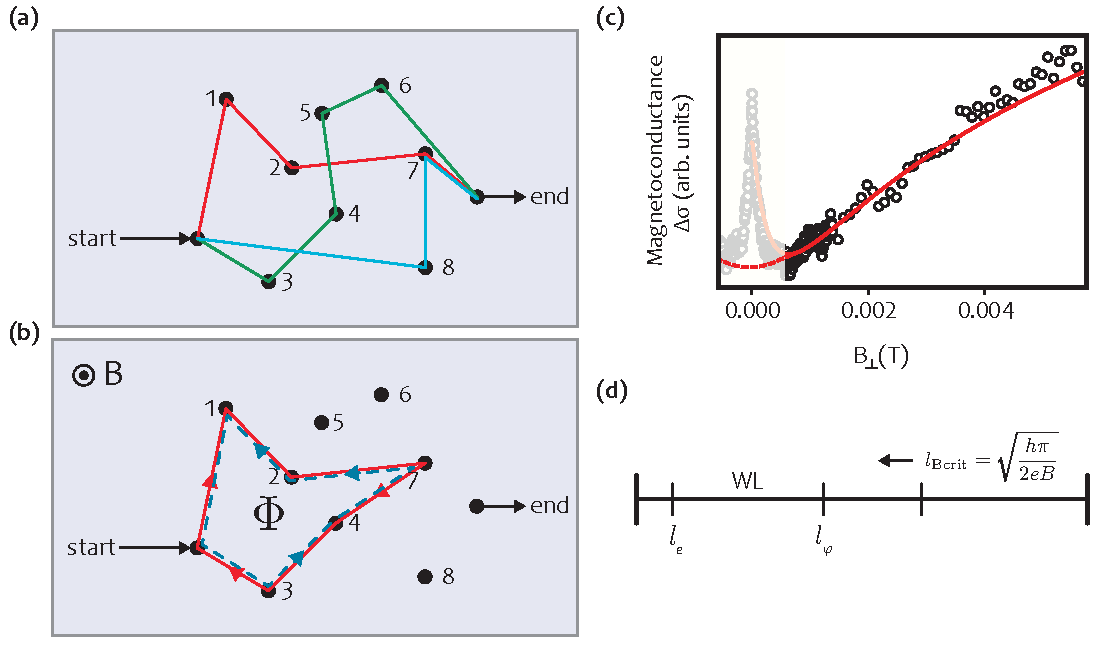
\includegraphics[width=0.85\linewidth]{wl}
  \caption[Weak localization]
  {\label{fig:WL}(a) To calculate the probability of transmission, we must sum together the wavefunctions for each path through the 2DEG. Scattering sites are represented by numbered dots, and several example paths are highlighted.
  (b) We can also calculate the probability that an electron will return to its starting location in the same way. Since an electron can travel in both a clockwise and counter-clockwise direction along the loop, there is an increased probability of reflection relative to transmission.
  (c) Weak localization in an InAs Hall bar. A weak anti-localization peak is seen at zero magnetic field, however, at small magnetic fields, weak localization begins to dominate, and we see a drop in conductance and a gradual recovery with the field as expected. (d) The relevant length scales in the weak localization problem. Weak localization is suppressed as the magnetic length is reduced (the field is increased).}
\end{figure}

Here $t_j$ is the transmission probability along the path $j$, and $\varphi_j$ is the phase accumulated along the path $j$.
The probability of finding the election at the endpoint is, therefore:
\begin{equation}
  P(\textrm{end}) = \left|\Psi_{\textrm{start}\rightarrow\textrm{end}}\right|^2 = \sum_j t_j^2 + \sum_{j \neq k} t_jt_k \cos(\varphi_j - \varphi_k)
\end{equation}
where the first term gives the probability of the electron travelling along a given path $j$, and the second term gives the
interference between each pair of paths through the lattice. Since the phases accumulated along each path are effectively random,
this second term will average to zero, and the total forward probability is given by:
\begin{equation}
P(\textrm{end}) \approx \sum_j t_j^2
\end{equation}
Next, let's consider paths that return to the starting point. In this case, we have both a clockwise and a counter-clockwise propogating
path (which we can label $j_+$ and $j_-$), around which, due to the symmetry of elastic scattering, we have the same transmission
probability $t_{j_+} = t_{j_-} = t_j$, and the same acquired phase $\varphi_{j_+} = \varphi_{j_-} = \varphi_j$. This situtation is represented schematically
in Fig.~\ref{fig:WL} (b). The return probability is therefore:
\begin{equation}
  P(\textrm{start}) = \sum_j \left(t_{j_+}^2 + t_{j_-}^2 + t_{j_+}t_{j_-}\cos(\varphi_{j_+} - \varphi_{j_-}) + t_{j_-}t_{j_+}\cos(\varphi_{j_-} - \varphi_{j_+})\right) = 4 \sum_jt_j^2
\end{equation}
In other words, \textquote[\cite{delftbook}]{phase-coherent summation of time-reversed trajectories in a diffusive medium leads to an increased probability for electrons
to return to their initial position}. To find an expression for conductance, we must find an expression for the probabilities of different paths, and take
into account the ratio of elastic and inelastic scattering length (the longer the path, the higher the chance that its phase will be randomized). A full derivation
is not given here, I will simply quote the final result, however I point the interested reader towards \cite{delftbook,datta1997electronic}. The correction
to conductance is given by:
\begin{equation}
  \Delta \sigma_{2D} = -\frac{1}{4\pi}\frac{2e^2}{h}\ln\left(\frac{l_\phi}{l_e}\right)
\end{equation}
As expected this gives us an reduced conductivity due to the increased probability of coherent back-scattering.

To extract a useful parameter from this, we need some way of differentiating the contribution of weak-localization from
the bare conductivity. To do this, we may apply a magnetic field perpendicular to the plane of the 2DEG, to break the time-reversal symmetry of the paths. For a magnetic field $B_\perp$, the phase difference along clockwise and counter-clockwise paths
is given by:
\begin{equation}
  \Delta \phi(B_\perp) = 4 \pi \frac{\Phi}{\Phi_0} = 4\pi \frac{B_\perp A}{\Psi_0}
\end{equation}
At the point where the magnetic field induces a $\pi/2$ phase shift around a loop, the destructive interference will be suppressed, thus the
effect of longer loops will be suppressed as a magnetic field is applied. A measurement of weak localization on an InAs Hall bar is shown in
Fig.~\ref{fig:WL}. Near zero field, there is a weak-antilocalization peak, a topic we cover in Sec.~\ref{sec:SOI}, however for fields
slightly above zero we see the reduction in conductivity and gradual increase towards the bulk value we expect.
Assuming paths are roughly circular we can approximate the length scale that a $\pi/2$ phase change between forwards and backwards
propagating paths corresponds to as:
\begin{equation}
  l_\textrm{Bcrit} = \sqrt{\frac{h \pi}{2 e B}}
\end{equation}

We therefore expect weak-localization to start getting suppressed when $l_\textrm{Bcrit} \approx l_\phi$, and the conductivity to return to the bare
value when $l_\textrm{Bcrit} \approx l_e$. This is shown in Fig.~\ref{fig:WL} (d). The exact form for the correction for weak localization unfortunately does not have
a simple form \cite{PhysRevB.70.245311}, however for a diffusive approximation, where $l_e \ll l_\phi$, we can use the reasonably simple form
given by \cite{10.1143/PTP.63.707}:
\begin{equation}
  \Delta \sigma_{2D}(B_\perp) = -\frac{2 e^2}{\pi h}\left[\digamma\left(\frac{1}{2} + \frac{B_0}{B_\perp}\right) - \digamma\left(\frac{1}{2} + \frac{l_e}{l_\phi}\frac{B_0}{B_\perp}\right)\right]
\end{equation}
where $\digamma$ is the digamma function and
\begin{equation}
  B_0 = \frac{v_F m^{*2}}{2 h e l_e n_s}
\end{equation}

Note that the diffusive approximation may not hold for high mobility GaAs samples, where the elastic scattering length is large.
Alternate forms are available in~\cite{PhysRevB.70.245311} which may be required for such samples.

\subsection{The Quantum Hall Effect}
As the field perpendicular to the sample is applied, which for brevity we will call $B$, apart from a modification to conductivity
we can also ask what occurs to the Hall (perpendicular) voltage and conductivity. As we saw in the Equation~\ref{eq:driftv},
the application of an electric field leads to a drift velocity in the sample set by the scattering
time $\tau$ and the effective mass of electrons $m^*$. In combination with the magnetic field $B$, this leads to a Lorentz force $F = e \vec v \times \vec B$, causing
a charge build-up along one edge of the Hall bar. The charge build-up is balanced out by an opposing electric field that is formed:
\begin{equation}
  E_y = -e \vec v \times \vec B
\end{equation}
To find the Hall resistivity, we can combine the electric field with the equation for current density, given in Equation~\ref{eq:currden}, to find
\begin{equation}
  \rho_{XY} = \frac{E_y}{J_x} = \frac{B}{n_s e}
\end{equation}
Hence, we find a linear relationship between magnetic field and Hall resistivity with a gradient proportional to the electron density, as seen in Fig.~\ref{fig:hall}.

As the magnitude of the magnetic field is increased, electrons are curved into roughly circular paths, with a radius:
\begin{equation}
  R_c = \frac{m^* v_F}{e B}
\end{equation}
and an angular frequency of:
\begin{equation}
  \omega_c = \frac{v_F}{R_c} = \frac{e B}{m^*}
  \label{eq:cycl}
\end{equation}
Once we are in the limit that $R_c \ll l_e$, we can write down a hamiltonian for the system:
\begin{equation}
  H = \frac{(P + eA)^2}{2m^*} + U(x, y)
\end{equation}
where $P$ is the momentum operator, and $A$ is the magnetic vector potential. We can choose the gauge of the vector potential such
that:
\begin{equation}
  \vec{A} = (0, Bx, 0)
\end{equation}
and expand the Hamiltonian, ignoring the Z component as we only have a single mode:
\begin{equation}
  H = \frac{p_x^2}{2m^*} + \frac{(p_y + eBx)^2}{2m^*}
\end{equation}

We note that the Hamiltonian is translationally invariant in the $y$-direction and can be rewritten as:
\begin{equation}
  H = \frac{p_y^2}{2m^*} + \frac{1}{2}m^*\omega_c^2(x - x_0)^2
\end{equation}
where we've substituted $\omega_c$ from Equation~\ref{eq:cycl} and $x_0 = \tfrac{p_x}{eB}$.

This Hamiltonian corresponds to that of a harmonic oscillator centred at $x_0$ with energy levels
\begin{equation}
  E_n = \hbar \omega_c\left(n + \frac{1}{2}\right)
\end{equation}
This implies that at high field, and neglecting the effects of scattering, our density of states evolves to
a series of discrete delta functions, where each state is highly degenerate, filled up to the state $E_n < E_F$.
Each of these states is called a \textbf{Landau level}. This situation is described by the schematic in Fig.~\ref{fig:hall}.
As a brief comment on the effects of scattering, which we've ignored in our derivation thus far. For the case that the quantum Hall effect is beginning to appear, and $R_c \sim l_e, l_\phi$, the Landau levels become broadened, although the exact mechanism
by which this occurs is not yet resolved \cite{PhysRevB.90.035425, PhysRevB.82.075401}. Up to this point,
we have been neglecting the effects of spin. We can, however, trivially add it to our energies:
\begin{equation}
  E_n = \hbar \omega_c\left(n + \frac{1}{2}\right) \pm \frac{1}{2}g^* \mu_b B
\end{equation}

Finally, we introduce a parameter to describe the number of electrons per magnetic flux quantum, which corresponds
to the number of Landau levels below the Fermi energy:
\begin{equation}
  \nu = \frac{n_s}{B / \Phi_0} = \frac{n_s h}{e B}
  \label{eq:nu}
\end{equation}

As we've moved to the Landau level description of states inside the 2DEG, you might expect that the conductivity of the sample should also
be modified, as we now no longer have free states at the Fermi level. This intuition is indeed correct, and the bulk of a Hall bar in the quantum
Hall regime will be insulating. Current is carried at the edges of the sample, where the confining potential curves upwards, and Landau levels
intersect with the Fermi level \cite{PhysRevB.25.2185} as shown in Fig.~\ref{fig:hall}. This gives rise to a series of chiral, 1D channels that carry current around the edges
of the Hall bar. Since these edge states are directional, and edges flowing in the opposite direction are physically separated by the width of the Hall
bar, backscattering is strongly suppressed, and edges provide dissipationless transport, i.e. $\rho_{XX} \rightarrow 0$.

What about the Hall resistance, $\rho_{XY}$? The number of edges that will cut through the Fermi level is given by $N_\textrm{max} = \lfloor \nu \rfloor$, each of which
will contribute to the total conductivity. The total conductivity is the sum of the conductances of each of the channels. Let's assume a difference in the
chemical potential of both sides of $\delta \mu = \mu_2 - \mu_1$. The total current across the sample is given by the product of the velocity $v_n(E)$ and the density of states $\rho_{\textrm{1D},n}$.
\begin{equation}
  J = e\sum_n^{N_{\textrm{max}}} \int_{\mu_1}^{\mu_2} v_n(E)\rho_{\textrm{1D},n}(E) \mathrm{d}E
\end{equation}
By a similar line of reasoning to Equation~\ref{eq:raw2dden}, we calculate the 1D DOS to be:
\begin{equation}
  \rho_{\textrm{1D},n} = \frac{1}{2\pi}\left(\diff{E_n(k)}{k}\right)^{-1}
\end{equation}
And the velocity from quantum mechanics is simply:
\begin{equation}
  v_n(E) = \frac{1}{\hbar}\diff{E_n(k)}{k}
\end{equation}
Hence, the total current is:
\begin{equation}
  J = e\sum_n^{N_{\textrm{max}}} \int_{\mu_1}^{\mu_2} \frac{1}{h} \mathrm{d}E = \frac{e N_{\textrm{max}} \delta\mu}{h}
\end{equation}
This remarkable cancellation between the DOS and velocity is unique to 1D channels and leads to the emergence of the conductance quantum that
we alluded to in section~\ref{sec:qd}. The difference in chemical potential is related to the voltage by $\delta \mu = eV$, and the conductivity is therefore:
\begin{equation}
  \sigma = \frac{J}{V} = \frac{N_{\textrm{max}} e^2}{h}
  \label{eq:hallsigma}
\end{equation}

\begin{figure}
  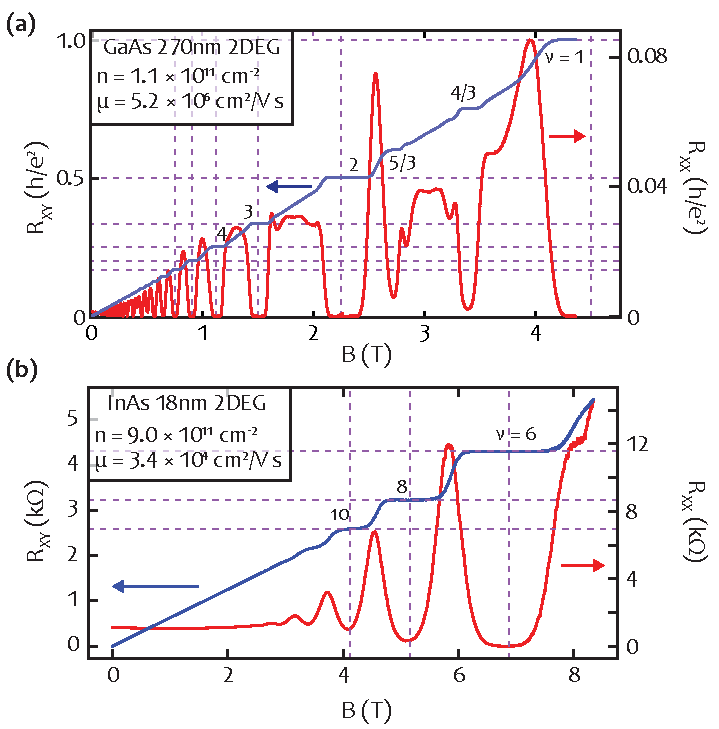
\includegraphics[width=0.7\linewidth]{hallcond}
  \caption[Integer quantum Hall effect in GaAs and InAs]
  {\label{fig:hallcond}(a) The integer quantum Hall effect in a high mobility GaAs 2DEG. The locations of filling factors are calculated using Eq.~\ref{eq:nu}
  and overlaid as dotted purple lines, while expected conductances are calculated using Eq.~\ref{eq:hallsigma}. (b) The same data except on an shallow InAs 2DEG.
  The higher density results in filling factors being shifted to higher magnetic fields. The lower mobility of the sample means plateaus are not visible up
  to high fields.}
\end{figure}

Therefore, we find the conductance of the edge will be quantized in units of the conductance quantum, with a value determined
by the filling factor, which gives us the number of conducting 1D channels parallel to the edge in the samples. An example of this, showing both $\rho_{XX}$
and $\rho_{XY}$ is given in Fig.~\ref{fig:hallcond}.

\subsection{Edge Magnetoplasmons (EMPs)}
The edge states of the Hall effect support charge density excitations, that we term \textbf{edge magnetoplasmons} (EMPs).
Such edge excitations are distinct from bulk plasmon (drum) modes and propagate with
a distinct frequency and dispersion that is set purely by the properties of the edge. Classical descriptions for such excitations
were first given in the 1980s, on 2DEGs formed on the surface of liquid Helium \cite{PhysRevLett.54.1706,PhysRevB.32.7676,1985ZhPmR..42..450V}.
We can understand the existence of such modes in a semiclassical picture. Consider a 2DEG running along the $x$ direction, placed in a magnetic field,
where the confining potential $E_y$ causes the appearance of edge states. A local perturbation, such as a gate voltage, can cause a dipole to form across
the sample, leading to an electric field that induces a propagating current $J = \sigma_{XY}E$ around the edge. As electrons are confined to travel at an
angle $\theta_H = \SI{90}{\degree}$ with a given directionality; this creates a self-propagating charge density wave (and hence electric current), that propagates
around the edge, a situation sketched in Fig.~\ref{fig:EMP} (a). Substituting Equation~\ref{eq:hallsigma} and Equation~\ref{eq:nu} into our expression for current density we find:
\begin{equation}
  J = n_s e \frac{E}{B}
\end{equation}

\begin{figure}
  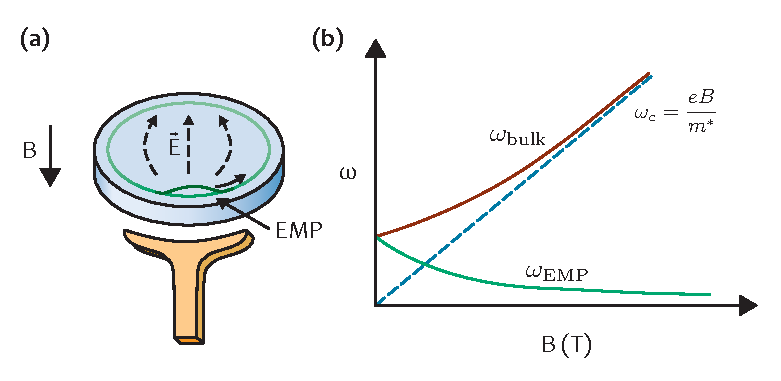
\includegraphics[width=0.65\linewidth]{EMP}
  \caption[Edge magnetoplasmons]
  {\label{fig:EMP}(a) Schematic of edge magnetoplasmon propagation. An external magnetic field is applied pointing into the Hall droplet.
  (b) Frequency of the EMP $\omega_\textrm{EMP}$ mode and bulk plasmon $\omega_\textrm{bulk}$ mode in a circular quantum Hall droplet with increasing magnetic field. At a high magnetic field, the bulk mode approaches the cyclotron frequency, while the edge mode has an approximately
  $1/B$ dependance on the field.}
\end{figure}

The resultant oscillatory modes are confined to the perimeter of the Hall sample and travel with a phase velocity $v_D$ approximated by the ratio
of electric and magnetic fields at the edge. To find the frequency of the EMPs, the details of the confining potential and edge must be calculated.
From \cite{1988ZhETF..94..217V}, the excitations are found to have a fundamental angular frequency of:
\begin{equation}
  \omega_{\textrm{EMP}} = \frac{\sigma_{XY}}{P\epsilon_0\epsilon^*}\left(\ln\left(\frac{P}{\pi w}\right) + C\right)
\end{equation}
where $P$ is the length of the edge, $\epsilon^*$ is the effective dielectric constant seen by the edge and C is a constant related to the geometry of the edge and goes to $1$ for a sharply defined edge with a step-like profile. The logarithmic correction arises due to electron correlations (which has a small impact,
unlike in other calculations), and $w$ represents the damping and physical width of the EMP from the edge:
\begin{equation}
  w = i\frac{\sigma_{XX}(\omega)}{2\omega\epsilon_0\epsilon^*}
\end{equation}
Note that this quantity does not necessarily go to zero on plateaus.
In the limit of low transverse resistivity, ignoring electron-electron interactions ($\omega\tau \ll 1$), and taking the limit
that $\omega_{\textrm{EMP}} \ll \omega_c$, we can approximate this term as:
\begin{equation}
  w \approx \frac{n_sm^*}{2\epsilon_0\epsilon_r B^2}
\end{equation}
These equations collectively show that the EMP travels at a significantly reduced frequency, which decreases with field, roughly proportionally to $\tfrac{1}{B}$.
Comparing the EMP frequency to that of a bulk plasmon in Fig.~\ref{fig:EMP} (b), one sees that while the fundamental bulk plasmon frequency $\omega_\textrm{bulk}$
approaches the cyclotron frequency $\omega_c$, the EMP frequency $\omega_\textrm{EMP}$ decreases towards zero. This slow and directional propagation is exploited in
Section~\ref{sec:hallcirc} and Section~\ref{sec:spinhallcirc} to construct compact circulators.

\subsection{The Spin-Orbit Interaction}
\label{sec:SOI}
Within a solid, we've thus far assumed that the spin or an electron is independent of its motion through that semiconductor, apart from
a tangential mention in Sec.~\ref{sec:dotqubits}, where we discussed its usefulness in controlling spins in semiconductors. In reality, the
band structure of the semiconductor, which up to this point we've captured in a single parameter, the effective electron mass $m^*$ is shaped
by a coupling of the motion of electrons through the lattice and around atoms. For this thesis, I will not aim to give a general description of
the effect, which contributes to a whole host of effects such as the fine structure hydrogen and the heavy/light hole structure of GaAs,
but rather give an intuitive understanding of its origins in a semiconductor. Hence, the terms that
I introduce here should not be considered to apply generally, but rather is specific to conduction band electrons in direct band-gap semiconductors.
This treatment is partly derived from \cite{winkler2003spin,dyakonov2017spin}.

Firstly, as we are dealing with conduction band electrons, which have a net spin angular momentum of
zero ($\vec S = 0$), we do not have any band splitting from the atomic orbitals. Instead, the SOI effect in conduction band electrons comes from effective
potential seen by an electron. Consider an electron moving through an asymmetric potential within a semiconductor. The asymmetric potential leads the
electron to feel an effective electric field, which in the rest frame of the electron is equivalent to an effective magnetic field, which causes an energy difference
between different spin species at a given $k$-vector. The origins of the asymmetric potential seen by the electron is manifested in two distinct ways. The first is called structural inversion asymmetry and is caused by an asymmetry in the confining potential of the electron (for example the triangle well that confines the 2DEG). The second is called bulk inversion asymmetry and comes from the lack of crystal inversion symmetry in III-V and II-VI semiconductors. These two terms lead to the Rashba and Dresselhaus terms, respectively.

We can write down the Hamiltonian for an electron in the system, including terms for the Rashba and Dresselhaus SOI:
\begin{equation}
  \mathbf{H} = \frac{p_x^2 + p_y^2}{2m^*} + \frac{\alpha}{\hbar}(\sigma_xp_y - \sigma_yp_x) + \frac{\beta}{\hbar}(\sigma_x p_x - \sigma_y p_y) +
  \frac{\gamma}{\hbar^3}\left(\frac{d}{\pi}\right)^2 p_x p_y (p_y\sigma_x-p_x\sigma_y)
\end{equation}
where $\sigma_x$ and $\sigma_y$ are the Pauli operators on the spin of the electron. The first term in this equation is the free-electron Hamiltonian and gives the motion of the electron through the semiconductor as we've seen in Equation~\ref{eq:k2d}. The second term is the Rashba SOI term, characterized
by a strength $\alpha$ and linear in momentum, creating an effective magnetic field perpendicular to the momentum of the electron. The third and fourth terms
are the Dresselhaus terms, with strength characterized by $\beta$ for the term linear in momentum and $\gamma$ for the term cubic in momentum. The cubic term is
generally small relative to the two linear terms in both InAs and GaAs quantum wells and is normally ignored. For the linear Dresselhaus case, the effective magnetic field twists
as the momentum of the electron changes \cite{PhysRev.100.580}. The effects of these terms are to shift the energies of the two spin species at each point of the dispersion
relation, a situation illustrated schematically in Fig.~\ref{fig:SOI} (a) and Fig.~\ref{fig:SOI} (b). As the Rashba term is set by the shape
of the confining potential of the electrons in the 2DEG, it is also strongly tunable by the gate voltage, which can induce greater asymmetry in the confining potential.
We should also note that although we call the effect of SOI an effective magnetic field, it is not a true magnetic field as
it does NOT break time-reversal symmetry or introduce an asymmetry in the population of different spin species. As can be seen from an inspection of
Fig.~\ref{fig:SOI} (a) and Fig.~\ref{fig:SOI} (b), states at each energy come in the form of Kramers pairs, such that:
\begin{equation}
  E_\uparrow(\vec k) = E_\downarrow(-\vec k)
\end{equation}
As the origins of this effect lie in the potentials formed by the constituent atoms of the semiconductors, we find that heavy-element semiconductors
will have a stronger SOI. For applications that require a strong spin-orbit interaction, the use of heavy-element III-V or II-VI semiconductors, such
as InAs, InSb or CdTe is common.

\begin{figure}
  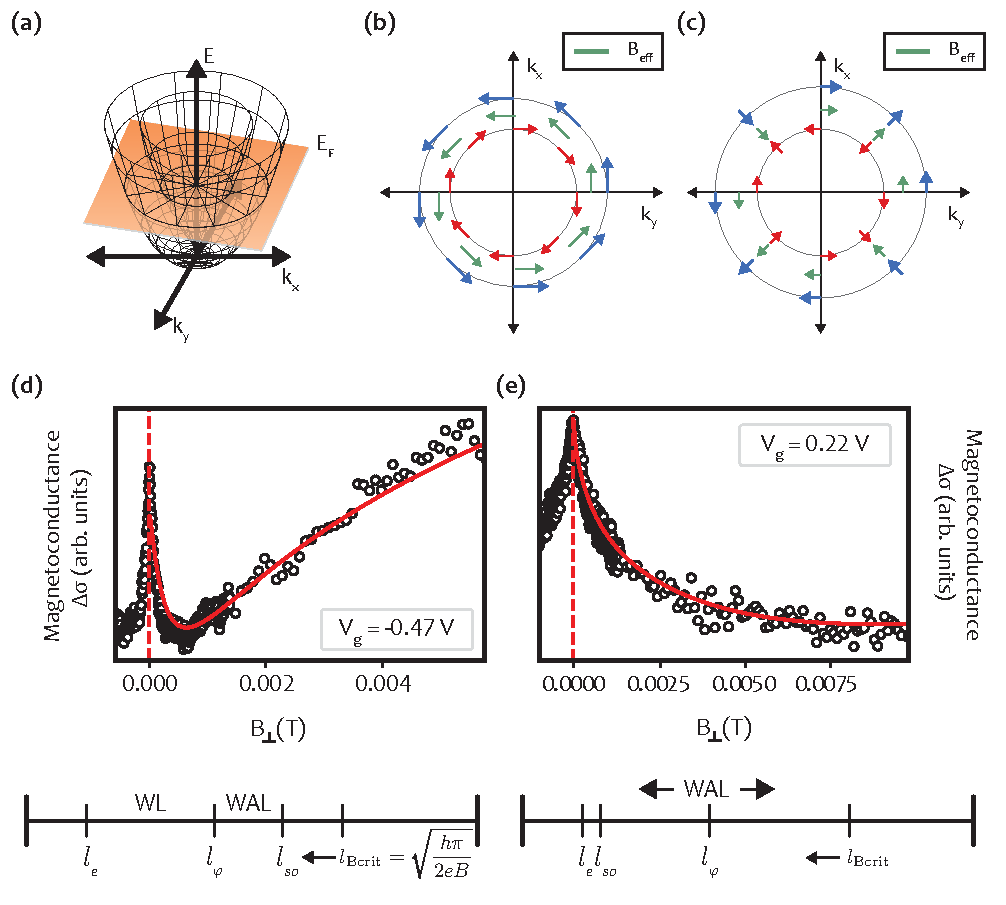
\includegraphics[width=\linewidth]{SOI}
  \caption[The spin-orbit interaction and weak anti-localization]
  {\label{fig:SOI}(a) The dispersion relation for a 2DEG under the influence of either Rashba or Dresselhaus SOI. Two offset parabolic dispersions are visible,
  a low energy and high energy spin branch. The Fermi energy $E_F$ is shown in orange cutting through the parabolas.
  (b) The dispersion relation at the Fermi surface under the influence of only the Rashba spin-orbit interaction. The effective magnetic field is shown in green. (c) The dispersion relation at the Fermi surface under the influence of only the Dresselhaus spin-orbit interaction.
  The effective magnetic field is shown in green. (d) Weak anti-localization and weak localization in an InAs Gall bar. In this case, $l_e < l_\phi < l_\textrm{so}$. A
  conductance peak is seen at zero field, which is rapidly suppressed by an applied perpendicular field. At intermediate fields, weak localization begins to dominate, leading to a dip and gradual rise in conductance. (e) Weak anti-localization in the same sample, for the case that $l_e \approx l_\textrm{so} < l_\phi$.
  The strength of the Rashba spin-orbit interaction is increased by the application of a higher gate voltage, leading to a tilted confining potential and
  a reduced spin relaxation length $l_\textrm{so}$.}
\end{figure}

Collectively, these effects allow us to engineer the Hamiltonians of our systems to generate topological phases of matter as we shall see in our discussion below,
where we use these effects to form anomalous quantum Hall states and Majorana zero modes. However, before we move onto those topics, we can close out our discussion of SOI
with a striking modification that SOI causes to weak localization as described in Sec.~\ref{sec:wl}. The fact that the rotation of spins occurs in opposite
directions for opposite momenta leads to destructive interference around self-intersecting paths. This leads to an increase in conductivity, or \textbf{weak anti-localization},
in materials with strong SOI \cite{10.1143/PTP.63.707}. However, as the electron scatters around a closed loop, the coupling of momentum and spin leads to the randomization of
the spin over several scattering events. In a semiconductor, this is described by the Dyakonov-Perel spin relaxation
mechanism \cite{DYAKONOV1971459}. We can, therefore, introduce a new length scale, $l_\textrm{so}$, the length over which a spin relaxes in a material with SOI.
This parameter is inversely proportional to the strength of the SOI, with a larger strength causing faster spin relaxation.
As the destructive interference relies on the differing energies between the two distinct spin species, the length scale over which spin relaxes in the semiconductor sets
a bound on the size of the loops where weak anti-localization can occur. As such, we are also able to measure
this effect via low-field Hall measurements in the same way we measure weak-localization, as seen in Fig.~\ref{fig:SOI} (c). Here the competition between
weak-antilocalization (peak) and weak-localization (dip) is visible as the field is swept on a sample of InAs with strong SOI. In this regime we have $l_e < l_\phi < l_\textrm{so}$
hence all three effects are visible. As the strength of the SOI interaction is increased by increasing gate voltage, the spin-orbit length becomes comparable to the elastic
scattering length $l_e \approx l_\textrm{so} < l_\phi$, thereby masking the effect of weak-localization, as seen in Fig.~\ref{fig:SOI} (d). For materials with only
Rashba SOI, the strength of the SOI may be extracted via fits given in \cite{10.1143/PTP.63.707}. For materials where both Rashba and SOI terms exist, a comprehensive
treatment of the correction to conductivity is given in \cite{PhysRevB.53.3912}.

\subsection{Quantum Anomalous Hall Effect}
One fundamental question we might ask is whether we can form edge states with quantized conductance that are protected from
scattering without an external magnetic field. It was several years before the question was answered in the affirmative by
Thouless \cite{PhysRevLett.49.405} and later Haldane \cite{PhysRevLett.61.2015}, their insight being the relationship between the
quantum Hall and related effects, and topology. For this insight, they were, along with Kosterlitz, awarded the Nobel Prize in 2016 \cite{nobel2016}.
Briefly, we can try and get an intuitive understanding of topology by considering the genus of an object. This is a global property of
a surface that is related to the number of holes in it. A ball, for example, has a genus of zero, and by continuous deformation, we can turn it
into other objects with the same genus, for example, a cube, a sheet of paper or even a pan have a genus of zero. A doughnut, on the other hand, has
a genus of one; it has a single hole. We can stretch and shape it into objects such as a mug, where the hole is its handle, but it can never become a ball.
This genus is captured by the Gauss-Bonnet theorem which states that the integral over the surface $S$ of a shape, with local curvature $K$ will yield
the genus $g$ of the object:
\begin{equation}
  \frac{1}{2\pi}\int_S K \mathrm{d}A = 2(1-g)
\end{equation}
We use a generalization of this theorem, called the Chern-Simons theorem, which allows us to map this theorem onto a band structure. We can define an
equivalent to "curvature" along the surface of bands in a solid, termed the Berrys phase. This is the phase that a particle travelling around
a path on the surface of a band acquires. The integral of the Berrys phase over momentum space leads to an integral quantity known as the Chern number
$n$, which is an integer and characterizes the topology of the material \cite{conmatphys-011417}. In the integer quantum Hall effect, the number $n$ is the same as the filling factor $\nu$, and gives us a topological explanation for the emergence of quantized edge states. As we transition from within
the material, with Chern number $n$, to free space, with Chern number $0$, there must be a twisting of the band structure near the edge that leads to the emergence of conductive edges. However, for the quantum Hall state, a large magnetic field is required to define the Berry's phase and hence the Chern number of the material.

In materials with a strong spin-orbit coupling, it is possible to find configurations with a non-zero Chern number, a topologically non-trivial band structure.
At the boundaries of such a material, a conductive state must appear \cite{PhysRevLett.93.156804,PhysRevLett.92.126603}, and indeed for heterostructures of \ce{HgCdTe}
the \textbf{spin quantum Hall effect} has been observed \cite{Konig766}, where two counterpropagating, spin-polarized, 1D channels lead to quantized conductance. Unfortunately, these
samples are sensitive to spin-scattering and thus have not been robustly demonstrated. The addition of a ferromagnetic dopant, such as chromium or vanadium lifts the
time reversal symmetry and generates leads to the formation of a spin-polarized chiral edge state, once the material has been taken past the coercive field of the
Cr or V dopants. This is termed the \textbf{quantum anomalous Hall effect}. The total conductance is given by the sum of the top and bottom edge states,
each contributing $e^2/2h$ of conductance, for a total Hall conductance of $\sigma = e^2/h$, as shown in Fig.~\ref{fig:qah}. We will use a sample that shows the
quantum anomalous Hall effect in Sec.~\ref{sec:spinhallcirc} to demonstrate a circulator that can operate without an external magnetic field.

\subsection{Forming Majoranas}
\label{sec:makemajo}

\begin{figure}
  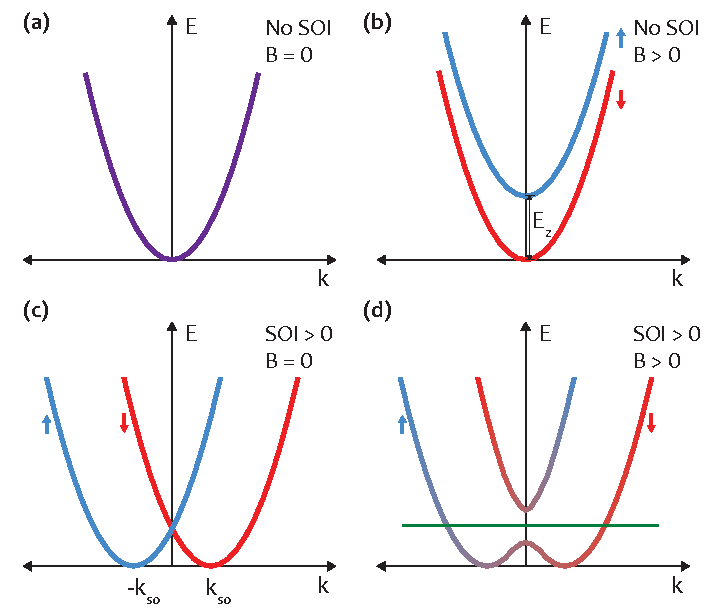
\includegraphics[width=0.75\linewidth]{1dSOI}
  \caption[Spin-orbit interaction in a nanowire with a magnetic field]
  {\label{fig:1dsoi}(a) The dispersion relation for a 1-dimensional chain of electrons (nanowire), assuming the nearly-free electron model. We obtain a parabolic band with two degenerate spin states. (b) The dispersion relation under the influence of an external magnetic field. A Zeeman splitting $E_Z$ occurs
  between $\uparrow$ and $\downarrow$ spins. (c) The dispersion relation in a material with either a Rashba or Dresselhaus spin-orbit interaction. The two spin species are shifted relative to each other by an amount $\pm k_\textrm{SO}$. Note that unlike a Zeeman field, this does not lead to any spin polarization in the material. (d) The dispersion relation in a material with spin-orbit interaction and an external magnetic field. The magnetic field creates a coupling between the split bands and opens a gap in the dispersion relation. If the chemical potential is tuned in the gap (green line) only a single band of the
  dispersion relation is accessible, equivalent to a system of spinless fermions.}
\end{figure}

In section~\ref{sec:majo} we went over a brief introduction to the physics that underpins quantum computation with Majorana zero modes
and left ourselves with the problem of finding a materials system that fits the model Hamiltonian given in equation~\ref{eq:kith}. I will stress
again that this Hamiltonian represents one proposed method of forming an emergent Majorana quasiparticle, there are many techniques described
in the literature involving a variety of materials systems, including in several excellent reviews \cite{RevModPhys.83.1057,doi:10.1146/030212-184337,Leijnse_2012,
RevModPhys.87.137,npjqi.2015.1,Aguado:2017ofc}. The technique of using a proximatized superconductor/semiconductor hybrid with strong SOI was reviewed
recently in \cite{s41578-018-0003-1} and goes into far greater detail than I attempt to here. To briefly recap, our Hamiltonian required a 1-dimensional
chain of spinless fermions and a superconducting pairing gap. Section~\ref{sec:2deg} covered the method by which we
can form systems with reduced dimensions in semiconductors; the remaining challenges are to create spinless fermions and induce a superconducting pairing gap
in a semiconductor. The combination of superconductivity and spinless fermions is termed superconducting p-wave pairing \cite{Kitaev_2001}. We can tackle
each challenge one at a time.

First, let's attempt to form a system of spinless fermions. We can accomplish this using the spin-orbit interaction as described in
Sec.~\ref{sec:SOI}. In a 1D chain, assuming a single dominant source of spin-orbit interaction (either Rashba or Dresselhaus), the coupling between momentum
and spin induces a shift in the momentum parabolas compared to the case of no spin-orbit coupling. This is depicted in Fig.~\ref{fig:1dsoi} (a) in the case of a bare
dispersion relation, and Fig.~\ref{fig:1dsoi} (b) in the case of a shifted dispersion under the influence of Rashba or Dresselhaus SOI. In this case, there is
no coupling between the high and low energy branches of the dispersion relation. The application of a magnetic field parallel to the 1D channel opens a Zeeman energy
gap between the two spin species with magnitude $E_z = g^* \mu_B B_\parallel$, as shown in Fig.~\ref{fig:1dsoi} (c), for a case with no SOI. In the case that the
SOI is present in the sample alongside an external magnetic field, there is a coupling between the two branches of the dispersion relation, which opens a gap in the
spectrum, seen in Fig.~\ref{fig:1dsoi} (d). If the chemical
potential is tuned inside the gap (green line), there is only a single band crossing the Fermi energy, effectively describing a system with a spinless degree of freedom.
The strength of the SOI in the material sets the field required to open a pairing gap in the material, hence the requirement for a material with a large SOI, without
which the strength of the required magnetic field would be prohibitive, particularly when considering our second requirement: superconducting pairing.

The pairing term can be accomplished using the proximity effect of a superconductor, that is the hybridization of superconducting and metallic states
between a superconducting metal and a semiconductor when a transparent interface joins the two. The is caused by the differing band structures between
the two materials; there must be a gradual change between the gapless band structure of the semiconductor and the gapped structure of the superconductor.
While Cooper pairs may penetrate the semiconductor for many microns, with a distance set by the elastic scattering length which destroys the coherence
of pairs, for a hard-gapped band structure at the 2DEG it is necessary for the heterojunction to be grown close to the 2DEG, generally within the
superconducting coherence length. Without a hard gap, quasiparticles are able to destroy the information stored in our Majorana fermions. Even with such a close spacing,
the material must have also have high mobility, as disorder scattering suppresses p-wave superconductivity and destroys the topological phase \cite{PhysRevB.84.144526}.
To ensure there are few subgap states, the most recent experiments have also required in-situ epitaxially grown aluminium interfaces, as any impurities at the superconductor
semiconductor interface have been found to contribute to significant sub-gap conductance \cite{nnano.2014.306}.

The choice of materials used for the formation of a Majorana zero mode in a superconductor/semiconductor hybrid system must, therefore, meet each of these, sometimes
conflicting, requirements. A large SOI and Land\'e g-factor calls for a heavy element III-V or II-VI semiconductor; however, the majority of high-quality growth has occurred
in GaAs. InAs and InSb have recently shown high mobilities for buried 2DEGs \cite{PhysRevMaterials.2.104602,doi:10.1063/1.4993784}, however the requirement for a hard-gap necessitates growth close to the surface of the semiconductor where it is difficult to shield the 2DEG from scattering off surface impurities, an issue we
tackle in Sec.~\ref{sec:inas_hb}. Nonetheless, recent experiments have demonstrated ever higher quality materials and more definitive evidence of zero bias peaks, close
to the expected value of $2e^2/h$\cite{PhysRevLett.119.136803,nature26142}, leading to a great deal of optimism for future applications using such devices.
